\begin{abstract}
Three-dimensional layer codes combine local stabilizer checks with favorable
storage parameters. We specify a realization of the Williamson--Baspin
construction for Calderbank--Shor--Steane (CSS) inputs with check weights at
least two and prove that it preserves the encoded dimension. Every pure-$X$
logical class is accessible in each lattice layer, and every pure-$Z$ class
in each transverse plane. For balanced good inputs of length $N$, these
slabs give the optimal distance scaling $\Theta(N^2)$. A three-dimensional
gauging grid with constant edge multiplicity preserves static code distance.
For the same gauging construction, a bounded-thickness bridge between two
blocks instead admits a short logical cut. Finite simulations support this
contrast at low noise; separate routed circuits exhibit bridge fault distance
one on three inputs and recover the tested idle-memory distances on the
smallest blocks with a spanning grid. We give local gate and deterministic
resource-distillation constructions and derive space and depth bounds for a
universal architecture, conditional on stated uniform detector, composition,
and resource-locality hypotheses under local-stochastic Pauli noise.

\end{abstract}
\maketitle
\raggedbottom

\section{Introduction}
Quantum error-correcting codes must protect stored information and make that
information accessible to computation. These demands can pull in different
directions: a code with favorable storage parameters may still require costly
logical measurements or physical connections that are difficult to realize.
Three-dimensional layer codes provide a natural setting in which to address
this problem. The construction of Williamson and Baspin embeds a Calderbank--Shor--Steane (CSS) code into
a local network of surface-code sheets and defects \cite{WilliamsonBaspinLayerCodes}.
For balanced good low-density parity-check inputs of length $N$, the resulting
blocks have
\begin{equation}
 n=\Theta(N^3),\qquad K=\Theta(N),\qquad d=\Theta(N^2),
 \label{eq:parameters}
\end{equation}
with bounded-weight, geometrically local stabilizers. Here $n$ is the physical
block size, $K$ its number of logical qubits, and $d$ its distance. A
\emph{balanced good} input family has $n_{\rm in}=N$,
$m_X,m_Z=\Theta(N)$, $K=\Theta(N)$, and both input distances
$\Theta(N)$, with uniformly bounded row and column weights. The chosen
generator lists may be redundant. Geometric spacing is fixed independently
of $N$.

The central result of this work is a geometric interface for processing that
stored information.  We give an explicit lattice realization of the layer code
with explicitly specified check matrices, and show that every pure-$X$ logical class has a
representative on a single layer of the lattice and every pure-$Z$ class one in
a single transverse plane.  The layer can be placed at any height, and the
plane at any position, independently of $N$ and of the chosen logical
operator.  This converts an algebraic choice of logical Pauli into a
spatially localized measurement port.

We use this interface to formulate a universal fault-tolerant architecture on the
native three-dimensional nearest-neighbor lattice.  The argument has three
steps. A prefix-parity construction first produces the slab representatives.
Relative expansion of a cubic grid then gives a local gauging measurement with
distance $\Omega(d)$. Finally, repeated extraction, padded composition, and
encoded resource transfer give a complete circuit under local-stochastic Pauli
noise, subject to the uniform hypotheses stated in Sec.~\ref{sec:ft-main}. Figure~\ref{fig:overview} summarizes the architecture.

\begin{figure*}[t]
\centering
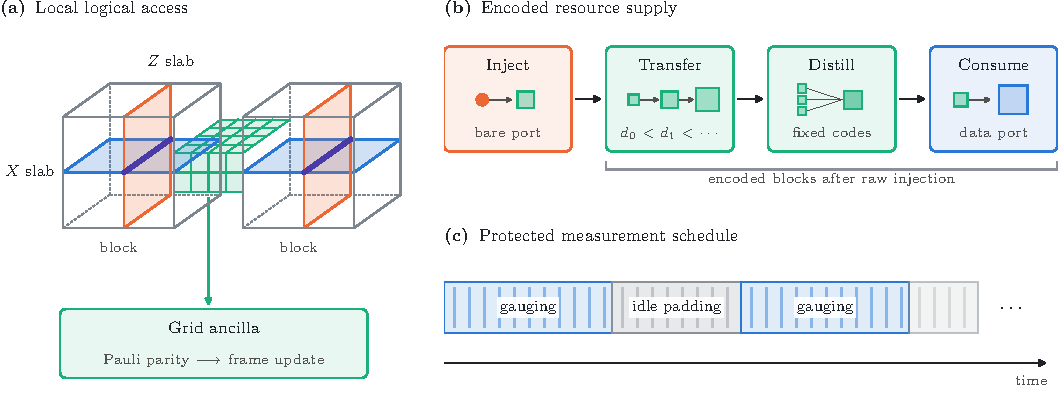
\includegraphics[width=\textwidth]{revision_architecture.pdf}
\caption{Geometry-preserving processing. (a) A layer-code block exposes
transverse slab ports for pure-$X$ and pure-$Z$ logical operators. A local grid
ancilla measures the selected Pauli; neighboring blocks use the same interface
for joint measurements. (b) A raw resource is injected into an encoded block,
transferred through blocks of increasing distance, distilled, and consumed by
the data path. (c) Repeated extraction and idle padding connect successive
active measurements. All drawings are schematic; the encoded blocks and grid
ancillas occupy three-dimensional regions.}
\label{fig:overview}
\end{figure*}

Logical measurement by gauging, surgery, and homological constructions has
become a general route to processing quantum LDPC codes
\cite{WilliamsonYoderGauging,CowtanParallelSurgery,YuanParsimonious2026,IdeHomological,BerentLiftedSurgery}.
Adapters, extractors, and universal architectures address complementary
questions of connectivity, parallelism, and resource overhead
\cite{SwaroopAdapters,HeExtractors,ZhangGoodQLDPC,MalcolmEfficientQLDPC}.
Here the organizing constraint is three-dimensional Euclidean locality:
logical access, resource delivery, and syndrome extraction use the same
nearest-neighbor geometry. The layer-code slab theorem supplies the missing
connection between the memory construction and these processing primitives.

Locality also fixes the achievable overhead. In three dimensions a local
stabilizer code obeys $Kd=O(n)$ \cite{BPT}, so $\Theta(d)$ physical qubits
per logical qubit is the best possible storage cost, and layer codes attain
it. Surface-code patches processed by lattice surgery use $\Theta(d^2)$
qubits per logical qubit \cite{HorsmanLatticeSurgery,LitinskiSurgery}, and
three-dimensional surface and color codes trade larger volume for
transversal gates \cite{VasmerBrowne}. Local simulations of LDPC codes
\cite{PattisonHierarchical}, local fault-tolerance constructions
\cite{ChoeKoenigLocal}, wire codes \cite{BaspinWire}, and planar logical
measurements \cite{YangPlanar} address related geometric questions, while
constant-overhead schemes
\cite{GottesmanFTThreshold,KovalevPryadko,FawziGrospellierLeverrier} and LDPC
magic-state injection \cite{ZhangInjectionIndependence,LiuInSituInjection}
rely on nonlocal connectivity. Under its stated uniform hypotheses, the architecture below keeps the
$\Theta(d)$-per-logical storage cost during computation, up to the cost of
one encoded cell for bounded-aspect logical boxes; general regions retain
a partial-occupancy correction.

This report proves the slab and static-distance results, specifies the local
logical primitives, and states separately the additional hypotheses needed
for the architecture bound. Section~\ref{sec:methods} specifies the lattice
and numerical protocol; Appendices~\ref{app:slab-proof}--\ref{app:conditional}
give supporting proofs and the precise conditional resource accounting.
Finite computations test the construction and interfaces; they do not
establish uniform properties of arbitrary adaptive schedules. Slab mobility
also gives the port-packing and shallow-unitary results of
Sec.~\ref{sec:structure}.

\section{Logical operators in constant-thickness slabs}
\label{sec:slabs}
\subsection{The layer code as glued sheets}
A layer code is assembled from surface-code sheets
\cite{WilliamsonBaspinLayerCodes}.  Each qubit $q$ of the input CSS code
becomes a \emph{data sheet}, the plane $y=Y_q$; each input $Z$ check becomes
a $Z$-check sheet, a plane $x=\mathrm{const}$; and each input $X$ check
becomes an $X$-check sheet, a plane $z=\mathrm{const}$.  Every sheet is an
ordinary surface code on a rectangle of the cubic lattice, so it carries
string operators.  An $X$ string joining the two boundary components on which its endpoints
condense commutes with all checks of that sheet; a string that
stops inside the sheet leaves a violated check, a \emph{defect}, at its end.
A $Z$-check sheet meets the data sheets of the qubits in its check along
vertical lines, the \emph{junctions}.  Ordered along the check, these are its
first, middle, and last junctions.  The $X$-check sheets are attached in the
same way, with $X$ and $Z$ exchanged.

A junction is a rule that says which strings may end on the line without
leaving a defect.  For the $X$ strings used below, only their presence
matters.  At a first or last junction the $Z$-check sheet ends on the data
sheet, and a string may pass from one sheet to the other: the check-sheet
string is present exactly when the data string is.  At a middle junction
three strings meet the line: the data string, which crosses it, and the
check-sheet strings on its two sides.  They leave no defect exactly when an
even number of the three is present.  Writing $1$ for a present string, and
listing the check-sheet strings first (left, then right) and the data string
last,
\begin{align}
 H_{\rm end}&=\begin{bmatrix}1&1\end{bmatrix}, &
 \ker H_{\rm end}&=\{00,11\},\nonumber\\
 H_{\rm mid}&=\begin{bmatrix}1&1&1\end{bmatrix}, &
 \ker H_{\rm mid}&=\{000,110,101,011\}.
 \label{eq:boundary}
\end{align}
Williamson and Baspin state these rules as sets of condensed anyons, that is,
as the combinations of string endpoints that disappear at the line;
Eq.~\eqref{eq:boundary} is the same information written for $X$ strings.  The word $110$ permits the pass-through needed below.  It lets a string on the check sheet pass a data sheet without
any string on that data sheet.  If a middle junction allowed only $000$ and
$111$, every check-sheet string would drag a string onto each data sheet it
passes, and a general logical operator could not be built; such a lattice in
fact fails to encode the input qubits (Table~\ref{tab:standalone-certificate}).

\subsection{An explicit lattice for the junctions}
We build every junction on the lattice (Sec.~\ref{sec:construction-details}).  Sheets own distinct qubits, and
each junction rule adds one qubit of one sheet to one check of the other.  At
a middle junction the $Z$-check-sheet face beside the line gains the data
sheet's edge on the line.  That face then contains three qubits of interest:
the check-sheet edge on the line, where the string from one side ends; the
next check-sheet edge, where the string on the other side begins; and the
added data edge.  Its check is therefore exactly the middle rule of
Eq.~\eqref{eq:boundary}.  The data stars on the line gain the check sheet's
edges on the same side, which keeps them commuting with the modified faces.
At a first or last junction the check sheet ends on the data line and shares
its edges, which gives the two-bit rule.

One more repair is needed.  An $X$-check sheet and a $Z$-check sheet cross
along a line, and there the junction additions of the two sheets make a few
stars and faces anticommute, once for each data qubit shared by the two input
checks.  A row of one-qubit additions along the crossing line, which we call
a \emph{wall}, removes these conflicts.  It exists exactly when the shared
number is even, which is the commutation of the two input checks.  The wall additions do not alter the slab commutation tests: the added
$a_y$ terms in $Z$ checks are absent from $X$ slabs, and the added $c_z$
terms in $X$ checks are absent from $Z$ slabs.
Every check lies within unit distance of one lattice vertex and has weight at
most six.  The junctions have the condensed anyons of
Ref.~\cite{WilliamsonBaspinLayerCodes}; we do not claim that the lattice is
identical to the drawings there, and all results below are proved for this
explicit lattice, specified in Sec.~\ref{sec:construction-details}.

\subsection{Slab representatives}

\begin{theorem}[Uniform slab representatives]
\label{thm:slabs}
For every input CSS code with checks of weight at least two, the explicit
realization encodes exactly $K$ logical qubits.  Every pure-$X$ logical class has a representative supported
on the single layer of $z$-edges spanning $[z_0,z_0+1]$, for every height
$z_0\in\{0,\ldots,L_z-1\}$ of the block, and every pure-$Z$ class has a
representative in the plane $x=x_0$, for every $x_0\in\{0,\ldots,L_x\}$.  The heights and planes are chosen independently of
the logical classes.
\end{theorem}

The operator is built at one fixed height $z_0$, one input check at a time.
Choose $x\in\ker H_Z$ of the input code, representing a pure-$X$ class
modulo $\operatorname{row}(H_X)$, and put an $X$
string at height $z_0$ on the data sheet of every qubit with $x_q=1$.  Each
such string crosses the junction of every $Z$-check sheet attached to its
data sheet, and on its own would leave a defect there.  Along one $Z$-check
sheet the selected junctions must therefore be joined, in pairs, by strings on
the check sheet at the same height; we call these check-sheet strings the
\emph{backbone}.  Pairing is possible because $x$ commutes with the input
check, so the check contains an even number of selected qubits.  Walk along
the check from its first qubit and switch the backbone on or off at every
selected junction.  With ordered incidences $x_1,\ldots,x_k$, the backbone
after the $i$th junction is present exactly when an odd number of selected
qubits lies behind it, a running count that we call the \emph{prefix parity},
\begin{equation}
 p_0=0,\qquad p_i=\sum_{h=1}^{i}x_h,\qquad p_k=0,
 \label{eq:prefix}
\end{equation}
where $p_k=0$ is the commutation $\sum_ix_i=0$ over $\mathbb F_2$.  At every
middle junction $p_{i-1}+p_i+x_i=0$, so none or two of the three strings are
present, as Eq.~\eqref{eq:boundary} requires; at the ends $p_1=x_1$ and
$p_{k-1}=x_k$.  No defect remains anywhere (Fig.~\ref{fig:slab-prefix}).
Every piece lies in the same layer of vertical edges, so the operator is one
lattice layer thick, whatever the block size and whichever logical is
chosen.  Building it at another height gives another representative of the
same class.  In the explicit realization the check is exact and local: every
stabilizer meets the operator in one of the forms $x_1+p_1$,
$p_{i-1}+p_i+x_i$, $p_{k-1}+x_k$ of a single incidence, or not at all.

\begin{figure*}[t]
\centering
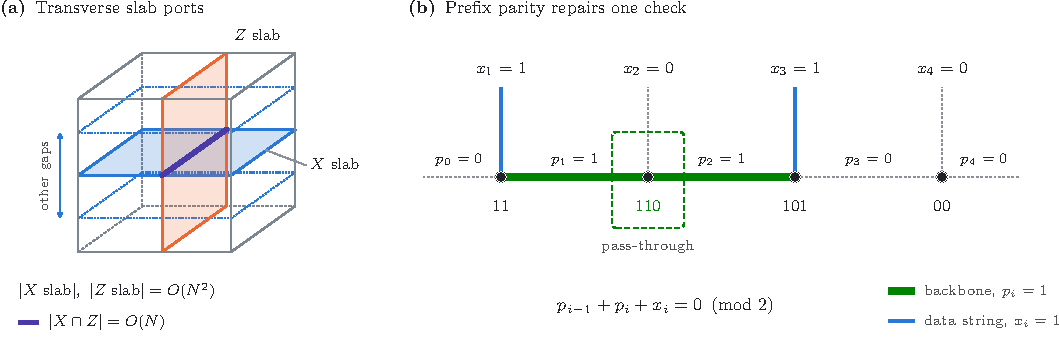
\includegraphics[width=\textwidth]{revision_slab_prefix.pdf}
\caption{Slab mobility and its local mechanism. (a) Complete $X$ and $Z$ ports
occupy transverse single-layer slabs. Each slab contains $O(N^2)$
qubits, and their intersection contains $O(N)$ qubits. Translating to another
height (or plane) gives another representative of the same logical class.
(b) For the even incidence word $(1,0,1,0)$, the running parity is
$(0,1,1,0,0)$. The highlighted middle cell uses $110$: the backbone remains
occupied although the data incidence is absent. Endpoint cells use the
two-bit relation in Eq.~\eqref{eq:boundary}.}
\label{fig:slab-prefix}
\end{figure*}

The pure-$Z$ operators are built in the same way in a vertical plane
$x=x_0$, with backbones on the $X$-check sheets.  An $X$ slab operator and a
$Z$ slab operator share only one data edge for each input qubit selected by
both, so they anticommute exactly when the two input logicals do.  This gives
$K$ independent logical qubits.  A count shows that there are no others.  On
its own, each data sheet would encode one qubit and each check sheet would
remove one; the junctions and walls add neither qubits nor checks; and every
redundancy among the lattice checks comes from a redundancy among the input
checks.  In formulas, each data sheet contributes $+1$ and each check sheet
$-1$ to $n-\#X-\#Z$, and the relations among the lattice checks inject into
those among the input checks.  Hence the realization encodes at most, and
therefore exactly, $K$ qubits, and the slab operators represent every
pure-type class.  Appendix~\ref{app:slab-proof} gives the relation maps and proves the
logical-space isomorphism, including redundant input checks and translation
of the slabs. Finite certificates on complete codes with up to $10{,}936$
qubits verify these properties on the tested instances
(Sec.~\ref{sec:verification-details} and Table~\ref{tab:standalone-certificate}).

Williamson and Baspin already obtain the layer-code logical operators by
quasi-concatenating input logicals \cite{WilliamsonBaspinLayerCodes}.  The
new ingredients are an explicit realization in which this construction can
be verified check by check, a single-layer thickness independent of the block
size and of the chosen logical, and its uniformity over every height, which
supplies the disjoint ports used below.

The same ports give the distance, by a simple idea: a logical operator must
be visible in every plane that contains a complete port of the other type.
Let $O$ be a nontrivial $X$ logical.  It anticommutes with some $Z$ logical,
and that $Z$ logical has a slab representative in each of the $L_x+1$
disjoint planes $x=x_0$, so $O$ must place qubits in every one of these
planes.  To count them, cut the $Z$ slabs of one plane into their pieces: a
vertical data column for each input qubit, and the backbone segments.
Record, for each piece, whether $O$ meets it an odd number of times.  Read a
data piece as its input qubit, and a backbone piece as the qubits of its
input $X$ check that lie behind it, the first $t$ of them for the $t$th
segment.  The resulting vector $\pi_{x_0}(O)$ commutes with every input $Z$
stabilizer because its pairing equals that of $O$ with the corresponding
lifted stabilizer. It pairs nontrivially with a conjugate input logical,
whose lift can be placed in this plane. Thus it is a nontrivial class in
$\ker H_Z/\operatorname{row}(H_X)$ and has at least
$d_X^{\rm in}$ entries (Appendix~\ref{app:slab-proof}).  The first $t$ qubits of a
check may be exchanged for the remaining ones, because the whole check is a
stabilizer of the input code, so a backbone piece stands for at most
$\eta_X=\max\{1,\lfloor w_X/2\rfloor\}$ qubits, where $w_X$ is the largest
input $X$-check weight.  Each piece met an odd number of times holds at least
one qubit of $O$, so each plane contains at least
$\lceil d_X^{\rm in}/\eta_X\rceil$ qubits of $O$, and
\begin{equation}
 d_X\ge(L_x+1)\left\lceil\frac{d_X^{\rm in}}{\eta_X}\right\rceil,
 \label{eq:distance}
\end{equation}
and, with $\eta_Z=\max\{1,\lfloor w_Z/2\rfloor\}$,
\begin{equation}
 d_Z\ge L_z\left\lceil\frac{d_Z^{\rm in}}{\eta_Z}\right\rceil.
 \label{eq:distance-dual}
\end{equation}
For balanced good inputs the realization therefore has
$n=\Theta(N^3)$, $K=\Theta(N)$, and $d=\Theta(N^2)$, the parameters of
Eq.~\eqref{eq:parameters}.  For the $[[4,2,2]]$ and $[[6,4,2]]$
inputs the bound equals the exact distance in every computed instance.

For balanced inputs the block has $\Theta(N)$ heights and $\Theta(N)$
transverse positions, so there are
\begin{equation}
 r_X=\Theta(N),\qquad r_Z=\Theta(N)
 \label{eq:mobility}
\end{equation}
pairwise-disjoint slab regions within each orientation. Each region is a
complete port for its logical polarization. This repeated access will also
give the structural bounds in Sec.~\ref{sec:structure}.

\section{Local gauging and universal logical operations}
\label{sec:measurements}
\subsection{Why a three-dimensional grid preserves distance}
Gauging measures a logical operator by measuring many small checks whose
product is that operator \cite{WilliamsonYoderGauging}.  Let
$\overline P=X(D)$ be the selected logical representative.  Attach each data
qubit of $D$ to its own vertex of a connected grid $G=(V,E)$, call these
vertices the \emph{ports} $U$, and place an ancilla qubit on every edge.  The
new check at a vertex, its \emph{vertex star}, is $X$ on the edges at that
vertex and on the attached data qubit, if any.  Every edge belongs to two
vertex stars, so the product of all vertex stars is $\overline P$, and the
product of their measured outcomes is the logical outcome; yet each
measurement involves only a few neighboring qubits.  The grid also carries
$Z$ checks around its unit squares, and every original $Z$ check that meets
$D$ is extended along short grid paths joining its ports, so that it commutes
with the stars.  Preparing the edge qubits in $|0\rangle$, measuring the new
checks, and finally reading the edges in $Z$ returns the data to its original
code with an updated Pauli frame.  The $X/Z$-exchanged construction measures
pure-$Z$ logicals.

The danger is that the added qubits create new, shorter logical operators.
The quantity that controls this is the expansion of the grid relative to its
ports,
\begin{equation}
 \beta(G,U)=\min_{\substack{S\subseteq V\\0<|S\cap U|<|U|}}
 \frac{|\delta S|}{\min\{|S\cap U|,|U\setminus S|\}},
 \label{eq:beta}
\end{equation}
where $\delta S$ is the set of edges leaving $S$ and only positive
denominators are included; throughout this lemma $|U|\ge2$. We call $\delta S$ a \emph{wall}: it separates
the ports in $S$ from the others, and $\beta$ is the smallest number of wall
edges paid per port separated.  For a code with CSS distances $d_X,d_Z$, the
deformed distances satisfy
\begin{equation}
 \widetilde d_X\ge\min\{1,\beta(G,U)\}d_X,
 \qquad \widetilde d_Z\ge d_Z.
 \label{eq:gauge-distance}
\end{equation}
The reason is short.  An $X$ logical of the deformed code may put part of its
weight on the ancilla edges, but those edges must form a wall $\delta S$;
any other edge set anticommutes with some square $Z$ check.  Multiplying by
the vertex stars in $S$ removes the wall and puts $X$ instead on the data
qubits attached in $S$, or, using the complement of $S$, on those attached
outside it.  Either way the result is a logical of the original code, so it
has weight at least $d_X$.  The trade removes $|\delta S|$ edges and, on the
better side, adds at most $m=\min\{|S\cap U|,|U\setminus S|\}$ data qubits,
while $|\delta S|\ge\beta m$.  Hence the deformed logical weighs at least
$\min\{1,\beta\}$ times a logical of the original code.  If $\beta\ge1$, no
logical saves weight by moving into the ancilla.  For the $Z$ sector, restriction to the original data maps a nontrivial
deformed logical class to a nontrivial original logical class. Indeed, if
the restriction is an original stabilizer, its deformed lift removes that
data support; the remaining ancilla support is a cycle and hence a
stabilizer. Ancilla support can be necessary for commutation, but cannot
reduce the weight of the data restriction. This proves
$\widetilde d_Z\ge d_Z$.

The slab geometry makes $\beta$ a constant, and this is where three
dimensions matter.  A slab representative lies in one plane and has
$\Theta(N^2)$ qubits, hence $\Theta(N^2)$ ports.  If the grid were only that
plane, a straight line across it would wall off half of the ports with
$\Theta(N)$ edges, so $\beta=O(1/N)$.  If the grid is a box as thick as it is
wide, a wall must be a surface.  Either it separates roughly the same region
in every layer of the box, and then it cuts through all the layers, or the
separated region changes from layer to layer, and every change costs edges
between layers.  In both cases its area grows in proportion to the number of
ports it separates.  If $U$
occupies at most $t$ parallel planes of a box with aspect ratio at most $A$,
Appendix~\ref{app:expansion} proves
\begin{equation}
 \beta(G,U)\ge\frac{1}{2At}.
 \label{eq:grid-bound}
\end{equation}
Constant refinement assigns distinct local port labels to distinct grid
vertices and increases $t$ only by a constant. Unit-square cycles, bounded
pairing paths, and bounded local density keep the check weight, diameter,
and incidence constant. Thus one block or two blocks at fixed bounded cell
separation admit local logical measurement using $O(n)$ ancillas and retaining
distance at least $\beta_0d$ for a fixed $\beta_0>0$. Section~\ref{sec:distance-floor}
shows that $\beta_0=1$ is attainable.

\subsection{Keeping the distance throughout the computation}
\label{sec:distance-floor}
A logical measurement can lower the fault distance, the smallest number of
faults that cause an undetected logical error, in three ways.  The added
qubits can carry a short logical operator; a few wrong measurement outcomes
can flip the reported result; and a few faults can exploit the join between
two consecutive operations.  Figure~\ref{fig:fault-distance} shows how the
construction blocks each of them.

The first danger is real for thin interfaces.  Consider a joint measurement
$\overline X_a\overline X_b$ of two blocks.  Once it has been measured,
$\overline X_a\overline X_b$ is a stabilizer, so $\overline X_a$ and
$\overline X_b$ act in the same way on the code.  Take any wall $\delta T$
with the ports of block $a$ on one side and those of block $b$ on the other.
The product of the vertex stars in $T$ is $\overline X_a$ times $X$ on the
wall, so $X(\delta T)$ alone is a logical operator equivalent to
$\overline X_a$ [Fig.~\ref{fig:fault-distance}(a)], and
\begin{equation}
 \widetilde d_X\le\min\{|\delta T|:\ T\cap U=U_a\}.
 \label{eq:cut-obstruction}
\end{equation}
For layer-code blocks of side $\Theta(N)$, the distance $d=\Theta(N^2)$ is
comparable to the area of a block face.  For these joint gauging measurements, assume bounded local qubit density
and edge multiplicity and a bridge of thickness $h$ and transverse extent
$O(N)$. A separating plane meets the bridge in $O(hN)$ edges. If
$\overline X_a$ survives as a nontrivial class after measuring the product,
Eq.~\eqref{eq:cut-obstruction} bounds the deformed static distance by
$O(hN)$. This is a cut obstruction for the specified gauging graph.  Joint measurements cannot be avoided: they implement
CNOT, phase teleportation, and resource transfer. A complete circuit-level
simulation on explicit layer-code blocks
(Sec.~\ref{sec:numerics-main}) finds the same effect in the fault distance of
the measurement circuit, exactly at two block sizes and, with routed
nearest-neighbor extraction, for three input codes, and in its failure rate
at four sizes.

\begin{figure*}[t]
\centering
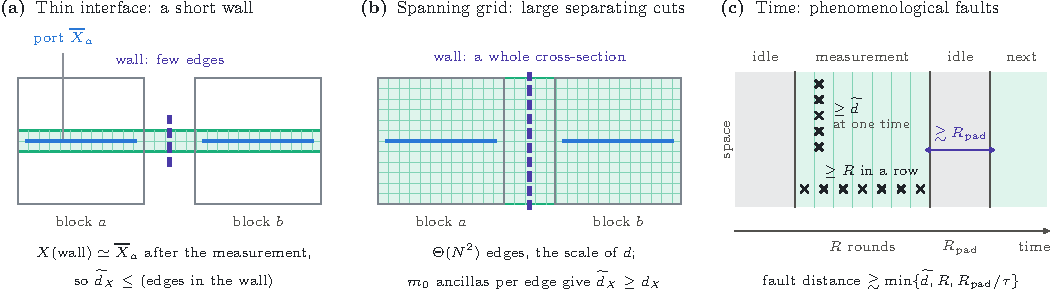
\includegraphics[width=\textwidth]{fault_distance_intuition.pdf}
\caption{Spatial and temporal mechanisms for distance protection.
(a) For joint gauging with a thin separating bridge, the cut operator is
equivalent to the surviving $\overline X_a$ class and bounds the static
distance. (b) Constant relative expansion and the complete cycle checks of
the amplified grid preserve static distance. (c) In the elementary
phenomenological model, the slice argument bounds detector-silent protected
faults by $\min\{\widetilde d_X,d_Z,R\}$. A measurement-only example flips
one star record in all $R$ rounds. General circuit faults require the
bounded-spread conversion, and composition requires the hypotheses in
Sec.~\ref{sec:ft-main}. The drawing is schematic.}

\label{fig:fault-distance}
\end{figure*}

Four ingredients keep the distance.  First, the grid fills the
participating blocks, so every wall between their ports is a surface with
$\Omega(N^2)$ edges [Fig.~\ref{fig:fault-distance}(b)]; this is the constant
relative expansion of Eq.~\eqref{eq:grid-bound}, which the constant slab
thickness makes possible.  Second, carrying $m_0=\lceil2At\rceil$ parallel
ancillas on every grid edge, with the square cycles on designated copies
and the weight-two parallel-edge cycles of Appendix~\ref{app:expansion},
multiplies every wall by $m_0$, so $\beta\ge1$
and Eq.~\eqref{eq:gauge-distance} gives $\widetilde d_X\ge d_X$: each
measurement keeps the full static distance at constant ancilla cost.  Third, the
measurement is repeated in time [Fig.~\ref{fig:fault-distance}(c)].  A single
wrong outcome of one vertex star flips the reported product, so the new
checks are measured for $R=\Theta(d)$ rounds, and a wrong outcome that is
not repeated is caught by comparing consecutive rounds.  In the measurement-only example, flipping one star record in all $R$
rounds changes the reported product without a consecutive-round detector.
Mixed data and record faults require a slice argument, rather than the
assumption that one fixed outcome is wrong in every round. In the elementary
phenomenological model a fault is one single-qubit Pauli or one record flip.
For a relative gauging rectangle with zero input error and zero output
syndrome and records, Appendix~\ref{app:slice} proves
\begin{equation}
 f_{\rm ph}^{\rm rect}\ge\min\{\widetilde d_X,d_Z,R\}.
 \label{eq:rect-distance}
\end{equation}
The argument retains arbitrary inherited error data by subtracting their
fault-free propagation. If each physical circuit fault has an equivalent
image of at most $c_1$ elementary mechanisms, then
\begin{equation}
 f_{\rm circ}^{\rm rect}\ge
 \left\lceil f_{\rm ph}^{\rm rect}/c_1\right\rceil.
 \label{eq:circuit-conversion}
\end{equation}
Thus static-distance preservation and circuit fault-distance preservation
are distinct statements. With bounded spread the resulting circuit lower
bound is $\Omega(d)$ when $R=\Theta(d)$. Fourth, padding successive
measurements by $\Theta(d)$ idle rounds supports composition under the
explicit conditions in Sec.~\ref{sec:ft-main}.

Resource transfer joins blocks of unequal distance. Let $C_1$ be the
smaller block and $C_2$ have distance at least $d_2$. For a joint $ZZ$
gauging measurement define $\mathcal Q_1$ as the subgroup of deformed
logical classes induced by logical operators of $C_1$ commuting with its
measured $\overline Z_1$; representatives are completed along grid edges
when required. The measured product identifies
$\overline Z_1$ with $\overline Z_2$ in this subgroup. The minimum weight
of a class outside $\mathcal Q_1$ is at least
$\min\{1,\beta\}d_2$ (Appendix~\ref{app:expansion}). This is a quotient
distance, not a lower bound on the entire two-block code. Dedicated courier
blocks carry one resource, with unused logical qubits in fixed states and
subsequently discarded. Protection of retained spectators during noisy
transfer also needs the relative propagation condition stated below.

\subsection{Gates and encoded resources}
Pure-$X/Z$ measurements suffice for the logical gate set. A CNOT uses an
ancilla $a$ in $|+\rangle$ and the measurements
\begin{equation}
 Z_cZ_a\;(u),\qquad X_aX_t\;(v),\qquad Z_a\;(w),
 \label{eq:cnot}
\end{equation}
followed by the Pauli-frame update $Z_c^vX_t^{u\oplus w}$.
Outcome bit zero denotes eigenvalue $+1$.

For phase teleportation, prepare $a$ in $R_\theta|+\rangle$, where
$R_\theta=\operatorname{diag}(1,e^{i\theta})$, measure $Z_dZ_a$ with bit $m$
and $X_d$ with bit $n$, and retain $a$. The correction
\begin{equation}
 C_{mn}=R_{2\theta}^{m}Z_a^nX_a^m
 \label{eq:phase}
\end{equation}
produces $R_\theta|\psi\rangle$. For $\theta=\pi/2$ this consumes
$|Y\rangle=S|+\rangle$; for $\theta=\pi/4$ it consumes
$|A\rangle=T|+\rangle$, with a possible $S$ correction using one additional
$|Y\rangle$. Exchanging $X$ and $Z$ gives $S_X=HSH$, and
$SS_XS=e^{i\pi/4}H$. These identities generate Clifford+$T$ using the
one- and two-block measurements above.

A physical resource enters at a designated bare port. The raw qubit is
teleported into an encoded block by a joint $ZZ$ measurement and an $X$
readout. Its weight-one error class is the intentional resource degree of
freedom; the static spectator quotient retains distance $\Omega(d)$. The
corresponding circuit statement uses the relative-transfer hypothesis in
Sec.~\ref{sec:ft-main}. Subsequent transfers use only encoded blocks, with
distances growing by fixed factors. We call this sequence an encoded courier.
Each courier block is dedicated to one traveling resource; its other logical
qubits are prepared in fixed states and never read.

The resource supply uses fixed Steane $7\!\to\!1$ and punctured Reed--Muller
$15\!\to\!1$ factories, implemented by the same logical primitives
\cite{BravyiKitaev,Reichardt,LitinskiMSD}.  Resource errors are modeled as local-stochastic defective slots. For any
set $J$ of preassigned candidate slots, the probability that all are
defective is at most $q_r^{|J|}$. Conditional on a defect set, good slots are
ideal product resource states; bad slots can be arbitrary and entangled
with one another or with an environment. This is a joint condition, not
merely a bound on each marginal error probability.

For phase teleportation with a defective resource, every conditional Kraus
operator, relative to the ideal rotation, lies in
$\operatorname{span}\{I,Z\}$. With an explicit environment the branch map
has form $I\otimes E_0+Z\otimes E_1$. The fixed recovery in
Appendix~\ref{app:factories} therefore returns the ideal output whenever at
most one coordinate of a run is defective. Each run always produces an
output, and disjoint runs obey the family bound
\begin{equation}
 q_{r+1}\le C_{\rm dist}q_r^2,\qquad
 C_{\rm dist}=\binom{30}{2}=435.
 \label{eq:distill}
\end{equation}
The 30 preassigned slots are fifteen principal candidates and fifteen
possible correction candidates. Unused candidates are discarded. The
one-defect property and the joint bound give a union bound over pairs for
each disjoint output run, without assuming independence or twirling.
Equation~\eqref{eq:distill} treats all other logical operations as ideal;
their physical faults must be covered separately by the architecture
hypotheses.

\section{Fault tolerance and resource scaling}
\label{sec:ft-main}
\subsection{From local distance to a complete circuit}
We consider local-stochastic Pauli circuit noise: any specified set $F_0$
of mechanisms at distinct circuit locations occurs with probability at
most $p^{|F_0|}$. A full architecture needs uniform properties of the
scheduled detector and effect maps, beyond the static-distance lemmas and
finite circuit checks. We state those properties explicitly.

At a temporal cut use $(s,\lambda,\rho)$ for the syndrome, logical Pauli
class, and last-round record error, all relative to a fixed ideal branch
and chosen Pauli representatives. These describe an error class, not an
arbitrary quantum state. For a fixed Clifford branch, the detector and
effect maps are binary linear maps on these variables and the internal
fault vector. Composition must carry all three variables; a faulty record
can change $\rho$ without changing $s$ or $\lambda$. Changing logical
representatives between cuts can add a term linear in $s$ to the propagated
frame. The relative effect of an internal fault vector subtracts the
fault-free propagation of the same incoming variables.

\begin{assumption}[Uniform scheduled-circuit hypotheses]
\label{ass:uniform}
There is a nearest-neighbor implementation with a fixed causal skeleton
and a finite set of adaptive branch templates satisfying the following
properties uniformly in block size, duration, and realized history.
\begin{enumerate}
\item A round has bounded depth and circuit-to-phenomenological spread
$c_1$. In the union of the branch detector catalogs, each detector involves
at most $a$ elementary mechanisms, each mechanism influences at most $b$
detectors, and at most $a_{\rm loc}$ mechanisms share a location. Edges
joining mechanisms in one detector or location have temporal range at
most $\tau$. All these constants are size independent.
\item Boundary maps compose exactly for arbitrary inherited
$(s,\lambda,\rho)$. A detector-silent component contained in an active or
idle window, with cuts in fault-free padding, has zero syndrome and
record error at its cuts. Its relative effect is its global contribution.
Relative distances obey $\delta_g^{\rm rel}\ge
\min\{\beta_0d,R_g\}$ and $\delta_{\rm mem}^{\rm rel}\ge d$.
At transfer boundaries, inherited errors on a courier, including its
syndrome and record terms, affect only its traveling resource and
discarded logical qubits; retained spectators obey the corresponding
large-block quotient bound.
\item Each retained block participates in at most one active window at a
time, with $R_{\rm pad}$ idle rounds between windows. A detector belongs
to one idle block or one active primitive; no detector joins distinct
lifetimes of a reused cell. Courier blocks are dedicated to one resource.
Distinct resource neighborhoods have union-graph separation $\Omega(R)$.
\item A committed minimum-cardinality decoder with a $\Theta(d)$ buffer
has the following witness property. A wrong protected commitment gives a
connected set of $\Omega(d)$ mechanisms with a fixed positive fraction of
actual faults. Except on a large-cluster event bounded by
$C V(C'p^{1/4})^{c d}$, wrong resource commitments have mutually disjoint
connected half-dense witnesses. Here $V$ is the total number of circuit
locations. A witness first created at courier stage $j$ has size at least
$\gamma d_j$ and an anchor set of size at most $C d_j^{5/2}$; the raw stage
has constant anchor size and witness size at least one. Terminal anchor
size is $O(f^{5/2})$, with witness size at least $\gamma d_J$.
\end{enumerate}
\end{assumption}

The relative distances refer to nonzero protected effect with zero
detectors and zero relative cut syndrome and records. They do not assign
distance $d$ to an unrestricted open cut: one late data fault can change
its syndrome. Appendix~\ref{app:slice} proves the elementary rectangle
bound under these boundary conditions. The uniform extension to arbitrary
adaptive histories, including the spectator propagation and decoder-witness
properties, is an additional hypothesis of the architecture result.
Finite schedule and single-fault checks do not discharge it.

Under Assumption~\ref{ass:uniform}, a detector-silent vector splits into
detector-silent connected components: all support vertices incident on one
detector are adjacent, so different components cannot cancel its parity.
Effects add on each fixed branch. A harmful component contained in one
window pays its relative distance. A component meeting successive
primitives on one block must cross the intervening idle pad. Consequently
\begin{equation}
 f_{\rm ph}\ge\min\left\{
 \min_g\delta_g^{\rm rel},\delta_{\rm mem}^{\rm rel},
 1+\left\lfloor\frac{R_{\rm pad}-\tau}{\tau}\right\rfloor
 \right\}.
 \label{eq:composition}
\end{equation}
The bound is used with $R_{\rm pad}>\tau$ and complete idle rounds at the
cuts. A component shorter than the padding term fits within one such
relative rectangle; the fault-free trailing round sets its cut records
and syndrome to zero. Choosing all full-distance windows and buffers of
order $d$ gives $\Omega(d)$ circuit distance after division by $c_1$.

Both incidence bounds in item 1 are necessary. They give fault-graph degree
at most $b(a-1)+a_{\rm loc}-1$; bounded detector support alone would not.
For fixed maximum degree, connected-set counting and the witness property
give exponentially small protected-failure probability. A geometrically
growing courier sequence gives a joint injected-resource parameter
$q_0=O(\sqrt p)$ by the charging estimate in
Appendix~\ref{app:conditional}. Thus the following theorem is a conditional
implication with explicit uniform hypotheses, rather than an inference
from finite simulations. Efficient classical decoding is not assumed.

\subsection{Architecture theorem}
The input family is a balanced good CSS LDPC family with boundedly dense
available sizes: every sufficiently large target length has an available
member within a fixed multiplicative factor. Fixed-degree Quantum Tanner
families provide the existential input used here
\cite{LeverrierZemorTanner,DinurLTC}. Let $A\subset\mathbb Z^3$ be the finite
allocated logical region, $W=|A|$, and $T$ the logical circuit depth. Allocated
working sites are included in $W$; physical gate ancillas and live factory
resources are included in the bound below.

To state the geometric overhead, partition the logical lattice into coarse
boxes of side $b(f)=\Theta(f^{1/6})$. Define $B_f(A)$ as the number of boxes
that meet $A$ but are not completely filled. This counts partial occupancy
at the block-packing scale, including boundaries, holes, and fragmentation.

\begin{theorem}[Conditional universal architecture]
\label{thm:architecture}
Use the explicit layer-code realization of Theorem~\ref{thm:slabs}, a
balanced good input family with boundedly dense sizes, and the local
measurement, resource, and extraction schedules satisfying
Assumption~\ref{ass:uniform}. There are constants
$p_{\rm th},c,f_{\min}>0$ such that for $0<p<p_{\rm th}$ and target failure
$0<\varepsilon<1/2$, any finite nearest-neighbor three-dimensional logical
circuit over Clifford+$T$, Pauli preparations and measurements, with
$W,T\ge1$, can be simulated with
\begin{equation}
 f=\max\left\{f_{\min},
 \left\lceil\frac{c\log(WT/\varepsilon)}{\log(p_{\rm th}/p)}\right\rceil
 \right\},
 \label{eq:f}
\end{equation}
using
\begin{align}
 Q_{\rm phys}&=O\!\left(Wf+(B_f(A)+1)f^{3/2}\right),
 \label{eq:space}\\
 D_{\rm phys}&=O(Tf^{3/2}\Psi),\qquad \Psi=O(f^{\log_215}).
 \label{eq:depth}
\end{align}
Here $W$ and $T$ are measured after compilation into this finite gate set;
$\varepsilon$ bounds implementation failure. If synthesis of other gates
is required, its approximation error and compilation overhead must be
allocated separately. Persistent data remain in layer-code blocks, and physical operations use
nearest-neighbor connectivity. For a connected bounded-aspect logical box,
\begin{equation}
 Q_{\rm phys}=O(Wf+f^{3/2}).
 \label{eq:box-space}
\end{equation}
\end{theorem}

The scaling follows directly from the code parameters. Choose
$d=\Theta(f)$ and measurement, padding, and commitment buffers of order $f$.
Equation~\eqref{eq:parameters} then gives
\begin{equation}
 N=\Theta(\sqrt f),\qquad K=\Theta(\sqrt f),\qquad n=\Theta(f^{3/2}).
 \label{eq:chosen-size}
\end{equation}
A full coarse logical box fits into one cell. Counting full and partial
boxes requires $O(W/K+B_f(A)+1)$ data/factory cells. Multiplication by
$n$ proves Eq.~\eqref{eq:space}. Neighboring logical sites map to the same
cell or adjacent cells, and a bounded coloring schedules inter-cell gates.



For a bounded-aspect logical box,
$B_f(A)=O((W/\sqrt f)^{2/3}+1)$, so the partial-cell term is absorbed into
Eq.~\eqref{eq:box-space}. The one-cell term dominates for $W\ll\sqrt f$;
the extensive term dominates for $W\gg\sqrt f$. Thin or fragmented regions
retain the general correction.

For time, a distilled resource takes $O(f\Psi)$ rounds, where $\ell$
distillation levels give $\Psi=O(15^\ell)$ and $2^\ell=O(f)$. One logical
layer requires $O(K)$ resources per data block, and serial production gives
$O(Kf\Psi)=O(f^{3/2}\Psi)$ rounds per layer, that is
$O(f^{3/2+\log_215})\subseteq O(f^{5.41})$. This serial schedule is chosen
to keep the space bound; parallel factories would trade space for depth. A depth-first factory schedule
stores $O(\ell)$ candidates at once, which fits within the reserved logical
capacity. The complete location count is polynomial in $f$ times
$WT\Psi$; the exponential cluster bound and final-resource union bound are
both at most $\varepsilon/2$ for the choice in Eq.~\eqref{eq:f}.


The depth deserves as much attention as the space. The serial schedule
takes $O(Kf\Psi)$ rounds per logical layer, so the storage advantage alone
does not establish a practical space--time advantage. In a bounded-aspect
logical box, $1\le P\le K$ independent resource lanes per data cell can,
under the same throughput and separation hypotheses, give
\begin{align}
 Q_{\rm phys}&=O\bigl(P(Wf+f^{3/2})\bigr),\nonumber\\
 D_{\rm phys}&=O\bigl(Tf\Psi\lceil K/P\rceil\bigr).
 \label{eq:parallel}
\end{align}
The factor $P$ includes factory cells even for a partially occupied data
cell. The ceiling retains a resource-latency floor. For $P\le K$ this gives
the same order of upper bound on qubit-time,
$O(Tf\Psi K(Wf+f^{3/2}))$; upper bounds do not imply equality of actual
costs. Hardware comparisons must include constants, routing, and decoder
costs. The architecture implication extends to another code family only
if it satisfies both the stated geometric properties and
Assumption~\ref{ass:uniform}.

\section{Port packing and shallow logical gates}
\label{sec:structure}
Slab mobility also constrains how logical information can be spatially
accessible. For a region $A$, let $g_X(A)$ be the dimension of the pure-$X$
logical space supported in $A$, and define $g_Z(B)$ analogously. The rank
$r(A,B)$ of their commutation pairing obeys
\begin{equation}
 \max\{0,g_X(A)+g_Z(B)-K\}\le r(A,B)\le |A\cap B|.
 \label{eq:overlap}
\end{equation}
The upper bound follows because all cross commutation factors through the
intersection; the lower bound follows from nondegeneracy of the full
logical $X/Z$ pairing.

If $A_1,\ldots,A_{r_X}$ are disjoint complete $X$ ports and
$B_1,\ldots,B_{r_Z}$ disjoint complete $Z$ ports, summing
Eq.~\eqref{eq:overlap} over all pairs gives the crossbar bound
\begin{equation}
 r_Xr_ZK\le n.
 \label{eq:crossbar}
\end{equation}
Every crossing carries rank $K$, and the crossings are pairwise disjoint.
For the balanced layer-code slabs,
$r_X,r_Z=\Theta(N)$, $K=\Theta(N)$, and $n=\Theta(N^3)$, so the bound is
saturated up to constants. Each transverse intersection has size
$\Theta(K)$, while each complete slab has size $\Theta(d)$. Thus the cubic
physical size is optimal among CSS families required to provide
$\Theta(K)$ disjoint complete ports in both polarizations. This is a bound
on simultaneous spatial access, distinct from a storage lower bound.

There is a complementary constraint on unitary processing. For a logical
Pauli $P=X(x)Z(z)$, pair the $i$th slab representative of $X(x)$ with the
$i$th representative of $Z(z)$. Each qubit belongs to at most two resulting representatives, giving
disjointness $\Delta=\Omega(N)$. The logical-weight bounds sharpen this to
\begin{equation}
 \Delta=\Theta(N),\qquad
 d_\downarrow=\Theta(N^2),\qquad d_\uparrow=\Theta(N^2),
 \label{eq:disjoint}
\end{equation}
where $d_\downarrow$ and $d_\uparrow$ are the smallest and largest minimum
weights among nontrivial logical Pauli classes. The
Jochym-O'Connor--Kubica--Yoder criterion then forces every fixed-depth,
bounded-arity, code-preserving unitary on a sufficiently large static block
to be logical Clifford \cite{JochymDisjointness}. The result holds even
without geometric locality of those gates. The architecture uses adaptive
measurements, resource states, and changing codes, which lie outside that
unitary setting.

\section{Finite numerical evidence}
\label{sec:numerics-main}
The supplied simulations test finite interfaces in the construction.  The
layer-code campaigns below use explicit blocks; the circuit-level campaigns with
a clean crossing use surface codes.
The largest campaign follows a single encoded planar surface code of distance
$L$, with $n=L^2+(L-1)^2$ data qubits, through an algebraic base-code
$\rightarrow$ gauged-strip $\rightarrow$ base-code circuit, without
resetting the data between stages. The gauged strip is a path of $L$
ancilla qubits attached to a weight-$L$ logical representative, so the
campaign tests the gauging interface and the detector bookkeeping of a code
switch rather than the layer-code geometry. Its entry and exit satisfy the binary
stabilizer transition identities. Noisy repeated extraction produces one
detector history, decoded by minimum-weight perfect matching using Stim's graphlike
decomposition of the circuit detector error model. The headline circuits
admit decomposition without ignored failures; this does not make a
matching decoder exact for correlated depolarizing faults. Physical shots
are sampled from the full circuit noise model.

The SI1000-like model uses two-qubit depolarizing strength $p$, single-qubit
and ordinary idle strength $p/10$, measurement flips $5p$, reset noise $2p$,
and data idle-wait noise $2p$. The archived campaign comprises 255 parameter
points and $4.534\times10^6$ shots for sizes $L=3,5,7,9,11$ and gauged
durations $G=d,2d,3d$, where $d=L$ is the code distance. All 15 noiseless controls have zero failures.

\begin{figure*}[t]
\centering
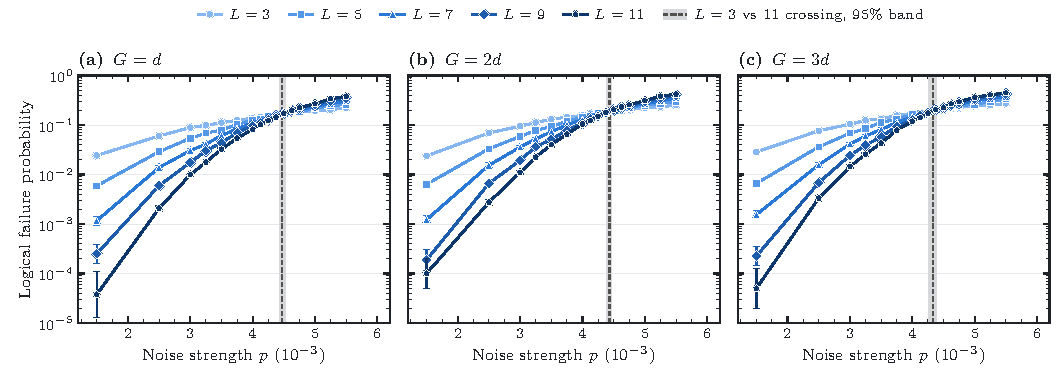
\includegraphics[width=\textwidth]{revision_numerics.pdf}
\caption{Finite algebraic code-switch diagnostics on the planar surface code
of distance $L$, redrawn from the archived shot counts. Panels (a)--(c) use
gauged durations $G=d,2d,3d$, respectively.
Markers identify the five sizes; bars are pointwise Wilson 95\% intervals.
Vertical dashed lines and shaded bands show the $L=3$ versus $L=11$ crossing
medians and conditional 95\% Jeffreys posterior intervals. The horizontal
axis is expressed in units of $10^{-3}$. These curves characterize the
implemented algebraic transition model; the bands show posterior uncertainty under the stated interpolation rule
and exclude systematic finite-size uncertainty.}
\label{fig:numerics}
\end{figure*}

For every duration, the failure rate decreases monotonically with $L$ across
all five sizes at every tested $p\le0.004$ (Fig.~\ref{fig:numerics}). Consecutive-size Wilson intervals are separated
at every tested $p$ from $0.0025$ to $0.00375$ for all three durations. At $p=0.0035$, increasing $L$ from 3 to 11 reduces the
failure rate from $0.1111$ to $0.0324$ for $G=d$, and from $0.1326$ to
$0.0428$ for $G=3d$. At $p=0.0015$ and $G=d$, the reduction is approximately
$6.5\times10^2$.

The smallest-versus-largest crossing medians are
$4.471$, $4.431$, and $4.328\times10^{-3}$ for $G=d,2d,3d$, with conditional
95\% posterior bands $[4.426,4.522]$, $[4.392,4.466]$, and
$[4.265,4.393]\times10^{-3}$. Tripling the gauged duration shifts the median
by about 3.2\%. These are finite-size diagnostics of a surface-code gauging model; they do
not estimate the architecture theorem's asymptotic threshold, which concerns
layer codes and a committed minimum-weight decoder.

A complete joint measurement on explicit layer-code blocks tests what the
surface-code campaigns cannot: the reported bit, both logical sectors,
spectator logicals, and an entangled input.  Two $[[4,2,2]]$-input blocks
($n=224$, two logical qubits each, distances $5$ and $4$) measure
$\overline X_1^{(a)}\overline X_1^{(b)}$ by gauging on a planar grid attached
to their single-layer slabs, with ancilla-based extraction of every check and
uniform circuit noise.  Each logical qubit starts maximally entangled with a
noiseless reference, and eight observables certify the output Choi state.
Without noise every detector and observable is deterministic, so the circuit
implements the projective measurement with the correct outcome and leaves the
spectators untouched.  We then minimize the number of faults that flips each observable
undetectably, reporting exact values or certified brackets according to
the solver status.  With a bridge of $w=1,2,3$ grid rows
between the blocks, the fault distance of
$\overline Z_1^{(a)}\overline Z_1^{(b)}$ is exactly $w$; for $w=1$ a single fault
suffices.  This is the cut obstruction of Sec.~\ref{sec:distance-floor} at
circuit level.  A grid spanning both blocks restores it to exactly $5$, the
blocks' $X$ distance, The reported-bit distance is $4$ and the tested spectator $X$-frame
distance is $4$ for all five interfaces. Several other distances remain
bracketed; Table~\ref{tab:all-distances} lists those bounds explicitly.

\begin{figure*}[t]
\centering
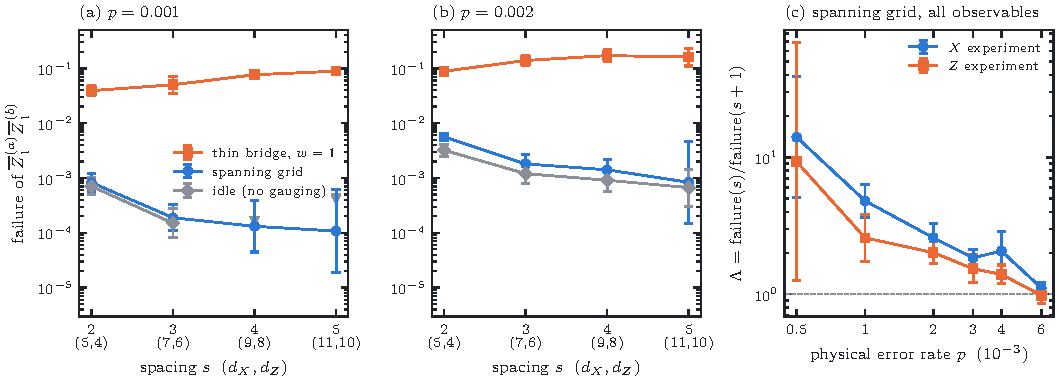
\includegraphics[width=\textwidth]{two_block_scaling.pdf}
\caption{Joint measurement at growing block size.  (a,b) Failure of the
measured pair's $Z$ sector through the one-row bridge, the spanning grid, and
for the same blocks idling without gauging, at $p=10^{-3}$ and
$2\times10^{-3}$; bars are Wilson $95\%$ intervals and open triangles the
upper end at zero failures.  At low noise the estimates show worsening bridge performance and overall
grid suppression compatible with idle memory; adjacent sizes need not
have statistically resolved differences.  (c) Suppression factor per unit
of spacing for the spanning grid (all observables of each experiment),
weighted fit over the available sizes with $95\%$ intervals; it reaches one
near $p\approx6\times10^{-3}$.}
\label{fig:standalone-scaling}
\end{figure*}

\begin{table*}[t]
\caption{Selected raw counts for the scaling experiment at $p=10^{-3}$:
failures/shots of the measured pair's joint $Z$ frame. Each block uses a
$[[4,2,2]]$ input, with $(d_X,d_Z)=(2s+1,2s)$ and $R=2s+1$ rounds per
phase. Idle controls run for the same $3R$ rounds without gauging.
Decoding is per-sector BP+LSD; $0/n$ has Wilson $95\%$ upper end about $3.8/n$.}
\label{tab:standalone-counts}
\centering\small
\begin{tabular}{@{}lrrrr@{}}
\toprule
Interface & $s=2$: $(5,4)$ & $s=3$: $(7,6)$ & $s=4$: $(9,8)$ & $s=5$: $(11,10)$\\
\midrule
One-row bridge & 78/2000 & 30/600 & 342/4500 & 252/2850\\
Spanning grid & 28/34000 & 13/69000 & 3/22800 & 1/9300\\
Idle control & 31/44000 & 10/66600 & 0/23400 & 0/9150\\
\bottomrule
\end{tabular}
\end{table*}

A second campaign repeats the measurement on blocks of spacing $s=2$ to $5$
(block distances up to $d_X=11$, up to $1400$ qubits per block), with $2s+1$
rounds per phase and $3.0\times10^6$ shots, decoded in each CSS sector
separately (Sec.~\ref{sec:simulation-protocol}); on identical
shots the full-model BP+LSD decoder has a lower estimated failure rate
through the grid (about half in the paired $X$ test) and a similar estimate
through the bridge at the tested points. This comparison is restricted to
those paired points.  At $p=10^{-3}$ the failure rate of
$\overline Z_1^{(a)}\overline Z_1^{(b)}$ through the one-row bridge rises from
$3.9\%$ at $s=2$ to $8.8\%$ at $s=5$, because the undetectable bridge fault
has more rounds in which to occur, while through the spanning grid it falls
from $8.2\times10^{-4}$ to about $10^{-4}$ and is statistically compatible with the estimates for the same blocks
left idle. This does not establish equivalence or a resolved improvement
at every successive spacing.  For the spanning grid each unit of spacing suppresses failures by
a factor $4.8$ in the $X$ experiment and $2.6$ in the $Z$ experiment at
$p=10^{-3}$, falling to one near $p\approx6\times10^{-3}$
(Fig.~\ref{fig:standalone-scaling}; raw counts in Table~\ref{tab:standalone-counts}).  At $s=3$ the fault distance of
$\overline Z_1^{(a)}\overline Z_1^{(b)}$ through a bridge of $w=1,2,3$ rows is
still exactly $w$, although the blocks' $X$ distance is now $7$.

A third campaign replaces the colocated ancillas by the routed
nearest-neighbor schedule of Sec.~\ref{sec:simulation-protocol}, with SWAP-shuttled ancillas,
colored conflict classes, and idle noise in every time step, and grows the
input at $s=2$: $[[4,2,2]]$, a six-qubit band code, and the Steane code,
giving blocks of $224$, $720$ and $1792$ qubits and circuits of up to
$16{,}293$ qubits.  Without
noise all $28$ measurement circuits implement the measurement exactly, and
the $12$ idle controls also give silent detectors and correct observables.  Through the one-row bridge the
fault distance of $\overline Z_1^{(a)}\overline Z_1^{(b)}$ is exactly $1$ for
all three inputs, although the blocks' $X$ distance grows from $5$ to at
least $18$.  On the $[[4,2,2]]$ blocks with $R=5$ rounds per phase
the spanning grid gives exactly $5$, the same as the blocks left idle;
through both interfaces the reported bit has exactly $5=R$, and the
spectator $X$ frames have exactly $4=d_Z$, as in idle memory.  Where both are
resolved, routing leaves the distances of the colocated circuit unchanged.
On the band blocks the reported bit has an undetectable pattern of weight $6$
at $R=7$.  The block itself explains this weight: the lightest $Z$-type
operator that anticommutes with the measured logical has weight $6$, and the archived circuit witness realizes weight six. Together with
the repeated-record witness, these bound the reported-bit fault distance
above by $\min\{R,6\}$ in this noise and measurement model; a smaller
routed-circuit minimum remains unresolved.  At the tested noise strengths the sampled
failure rates of these long routed circuits do not distinguish the
interfaces, so we report exact fault distances where certified and explicit bounds
otherwise.

The deterministic checks include the complete-code slab certificate and
negative controls in Sec.~\ref{sec:verification-details}. These support
the finite construction and remain separate from the arbitrary-size proofs.

\section{Discussion and conclusions}
The slab theorem gives a local route from layer-code storage to logical
access. Prefix-parity repair exposes logical operators in single-layer
slabs of an explicit realization, and amplified grid gauging preserves
static distance. The local primitives support universal logical operations
and deterministic resource distillation. Under the uniform scheduled-circuit
hypotheses, the architecture bound separates an extensive $Wf$ space cost
from the minimum $f^{3/2}$ cost of one encoded cell in bounded-aspect logical
boxes. Establishing these hypotheses for the full adaptive implementation
is a remaining proof requirement; the finite certificates verify only their
tested instances.

The next steps are a uniform proof of the scheduled detector, transfer,
and decoder-witness conditions; a practical decoder for deformation histories, with
changing checks, inherited frames and records, and joint measurements (the
layer-code decoders of Ref.~\cite{GuRandomLayerCodes2026} are a natural starting
point, although their memory guarantees do not yet cover code switching);
routed circuit-level benchmarks on inputs that grow into the balanced regime,
with a shorter routed schedule and a decoder close to minimum weight; bounds
on how many logical measurements can share
the slab interfaces, compared with parallel code surgery
\cite{CowtanParallelSurgery} under three-dimensional locality; and factories
whose constants make the space--time estimate competitive, possibly in a
different code with a protected local transfer. Random
layer codes built from random CSS inputs \cite{GuRandomLayerCodes2026} are a
natural candidate for reducing those constants; the explicit realization
applies to any CSS input, but the resource accounting would need their
parameter scaling. The conditional architecture theorem uses minimum-weight committed decoding and
local-stochastic Pauli noise. Extensions to coherent or leakage noise require
an additional fault-path analysis; deterministic selection of the input
component codes is a separate constructive problem. Comparing the space
bound with an extensive storage lower bound requires the restricted regime
$W=\Omega(\sqrt f)$, so that the one-cell term is not dominant.


\section{Construction and computational methods}
\label{sec:methods}
\subsection{Lattice specification}
\label{sec:construction-details}
Let $H_X\in\mathbb F_2^{m_X\times n_{\rm in}}$ and
$H_Z\in\mathbb F_2^{m_Z\times n_{\rm in}}$ be the check matrices of an input
CSS code with $H_XH_Z^T=0$, every check of weight at least two, and
$K=n_{\rm in}-\rank H_X-\rank H_Z$.  Fix an integer spacing $s\ge2$ and set
\begin{align}
 Y_q&=sq,\quad X_j=s(j+1),\quad Z_i=s(i+1),\nonumber\\
 L_x&=s(m_Z+1),\quad L_z=s(m_X+1),
 \label{eq:explicit-coords}
\end{align}
with $q=1,\dots,n_{\rm in}$, $j=0,\dots,{m_Z-1}$ and $i=0,\dots,{m_X-1}$.
For a check $c$ write $q_1^{(c)}<\cdots<q_{k_c}^{(c)}$ for its support in
increasing order; $q_1^{(c)}$ is its \emph{first}, $q_{k_c}^{(c)}$ its
\emph{last}, and the others its \emph{middle} incidences.

\paragraph{Sheets.}
Every sheet is an edge surface code on a rectangle of the cubic lattice: one
qubit per unit edge of the sheet, an $X$ check (\emph{star}) on each vertex
acting on the sheet edges at that vertex, and a $Z$ check (\emph{face}) on
each unit square acting on its boundary edges.
\begin{itemize}
\item Data sheet $D_q$ ($q=1,\dots,n_{\rm in}$): the plane $y=Y_q$ with
$0\le x\le L_x$, $0\le z\le L_z$.  The rows $z=0$ and $z=L_z$ carry no
$x$-edges and no stars.
\item $Z$-check sheet $C_j$: the plane $x=X_j$ with
$Y_{q_1}\le y\le Y_{q_k}$ ($q_t=q_t^{(Z_j)}$) and $0\le z\le L_z$.  The rows
$z=0,L_z$ carry no $y$-edges and no stars.
\item $X$-check sheet $A_i$: the plane $z=Z_i$ with
$Y_{q_1}\le y\le Y_{q_k}$ ($q_t=q_t^{(X_i)}$) and $0\le x\le L_x$; every
vertex carries a star.
\end{itemize}
Distinct sheets own distinct qubits, also on coincident lattice edges, with
one exception: the first and last $z$-edge columns of $C_j$ \emph{are} the
$z$-lines $(X_j,Y_{q_1},\cdot)$ and $(X_j,Y_{q_k},\cdot)$ of $D_{q_1}$ and
$D_{q_k}$, and the stars of $C_j$ on those columns are merged into the
corresponding data stars.  A sheet pair without an input incidence therefore
crosses transparently.  At most two qubits share a lattice edge.

\paragraph{Line junctions.}
Write $d_\mu(v)$, $c_\mu(v)$, $a_\mu(v)$ for the $\mu$-directed edge
$v\to v+\hat\mu$ of $D$, $C$, $A$ respectively.  The input incidences act by
adding one qubit to existing checks:
\begin{itemize}
\item[(Z)] for $q=q_t^{(Z_j)}$ and every vertex $u=(X_j,Y_q,z)$ of the
$z$-line: for $1\le z<L_z$, the final support of the $D_q$ star at $u$ contains $c_y(u)$ if $t<k$ and $c_y(u-\hat y)$ if
$t=k$; for $0\le z<L_z$, if $q$ is a middle incidence, the $C_j$ face on
$[Y_q,Y_q+1]\times[z,z+1]$ gains $d_z(u)$.  (For the first and last incidence
the adjacent $C_j$ face already contains $d_z$ through the shared column.
The endpoint star merge already includes the indicated $c_y$ edge; do not
add it a second time modulo two.)
\item[(X)] for $q\in\operatorname{supp}X_i$ and every vertex
$u=(x,Y_q,Z_i)$ of the $x$-line: the $A_i$ star at $u$ gains $d_z(u)$, and the
$D_q$ face on $[x,x+1]\times[Z_i,Z_i+1]$ gains $a_x(u)$ for
$0\le x<L_x$.
\end{itemize}

\paragraph{Walls on crossing lines.}
A $Z$-check sheet $C_j$ and an $X$-check sheet $A_i$ cross along the $y$-line
$\ell_{ij}=\{(X_j,y,Z_i)\}$ for $y$ in the overlap $[\ell,h]$ of their
$y$-ranges.  On this line we allow two further one-qubit additions, with
binary coefficients $\sigma_y$ ($\ell\le y\le h$) and $\tau_y$
($\ell\le y<h$): the $A_i$ star at $(X_j,y,Z_i)$ gains
$\sigma_y\,c_z(X_j,y,Z_i)$, and the $C_j$ face on
$[y,y+1]\times[Z_i,Z_i+1]$ gains $\tau_y\,a_y(X_j,y,Z_i)$.  The coefficients
are the unique solution of the commutation conditions of
the checks: the additions change the overlap of the $A$ star at $y'$ and
the $C$ face on $[y,y+1]$, $y'\in\{y,y+1\}$, by $\sigma_{y'}+\tau_y$.
All commutation equations, including those with checks immediately
outside the overlap and adjacent data faces, are imposed. If the $C$ face
on $[\ell-1,\ell]$ exists it fixes $\sigma_\ell$; if the overlap starts
at the shared first $C$ column, the adjacent $D$ faces force
$\sigma_\ell=0$. The right endpoint is handled in the same way. Empty
overlap requires no wall; a single-vertex overlap has only its one $\sigma$
and the endpoint equations, with no $\tau$. The resulting path has fixed ends; summing its equations gives
$|\operatorname{supp}X_i\cap\operatorname{supp}Z_j|$ modulo two. The system
is therefore solvable, uniquely, exactly when that overlap is even, which
holds for every CSS input. This completes the check-matrix specification.


\subsection{Complete-code verification and controls}
\label{sec:verification-details}
All finite checks use exact GF(2) linear algebra on the complete check
matrices; no boundary check is omitted. For seven input codes and spacings
$s=2,3$ where feasible, the tests verify commutation, solvability of every
wall system, the Euler count $n-\#X-\#Z=n_{\rm in}-m_X-m_Z$, the dimensions
of the relation spaces, and $k=K$. Table~\ref{tab:standalone-certificate}
records the resulting logical count and slab-pairing rank.

For each stabilizer, the overlap with the symbolic prefix operator is
compared with the first/middle/last forms of Eqs.~\eqref{eq:boundary}
and~\eqref{eq:prefix}, at every height and every dual plane. For a single
check of weight $2\le k\le6$, all $2^{2k-1}$ incidence/backbone assignments
are enumerated. Precisely the $2^{k-1}$ even incidence words with their prefix
backbones have zero syndrome; odd words and single-segment flips fail.
Every basis input is checked for stabilizer commutation, mapping of input
stabilizers to stabilizers, and preservation of the logical pairing.
Here HGP denotes a hypergraph-product code. The single-chart negative
control identifies every incidence column of a check sheet with the
corresponding data column, including middle incidences, thereby removing
the independent check-sheet pass-through channel. Its precise construction
is included in the source archive. For this control, its encoded dimension
differs from $K$ for every tested input. Walls with odd check overlap are
inconsistent; the even-overlap controls are solvable.

\begin{table}[t]
\caption{Complete-code verification. All rows have zero anticommuting
check pairs. The encoded dimension and slab-pairing rank both equal $K$;
the last column is the incorrect logical count of the single-chart control.}
\label{tab:standalone-certificate}
\centering\scriptsize
\setlength{\tabcolsep}{3pt}
\begin{tabular}{@{}lrrrr@{}}
\toprule
Input & $s$ & qubits $n$ & $k=$ pairing rank & control $k$\\
\midrule
$[[4,2,2]]$ & 2 & 224 & 2 & 4\\
$[[4,2,2]]$ & 3 & 504 & 2 & 4\\
$[[6,4,2]]$ & 2 & 352 & 4 & 6\\
$[[6,4,2]]$ & 3 & 792 & 4 & 6\\
Steane $[[7,1,3]]$ & 2 & 1792 & 1 & 10\\
Steane $[[7,1,3]]$ & 3 & 4032 & 1 & 10\\
Hamming $[[15,7,3]]$ & 2 & 6600 & 7 & 29\\
Surface $[[13,1,3]]$ & 2 & 10314 & 1 & 15\\
Random HGP 1 & 2 & 10936 & 2 & 20\\
Random HGP 2 & 2 & 10512 & 2 & 18\\
\bottomrule
\end{tabular}
\end{table}

\subsection{Simulation and inference protocol}
\label{sec:simulation-protocol}
\paragraph{Layer-code circuits.}
The initial two-block experiment has $12$ port qubits per block. Every
check is measured with its own ancilla and CNOTs, $X$ checks before $Z$
checks, for four rounds before, during, and after gauging. Grid edges are
prepared in $|0\rangle$ and read in $Z$; edge readouts update the Pauli
frame. Uniform circuit noise applies two-qubit depolarizing noise of
strength $p$ after each CNOT, one-qubit depolarizing noise on data and edge
qubits each round, and flips of probability $p$ after resets and before
measurements, including final readout. This differs from the SI1000-like
surface-code model specified in Sec.~\ref{sec:numerics-main}.

Every input logical qubit is entangled with a noiseless reference.
An $X$-basis experiment tests the reported parity and four logical $X$
frames; a $Z$-basis experiment tests the measured pair's joint $Z$ frame
and two spectator $Z$ frames. These eight observables certify the output
Choi state in the noiseless circuit. CP-SAT minimizes the number of undecomposed
detector-error mechanisms that flip a chosen observable with zero detector
syndrome. A distance is called exact only when optimality is proved;
otherwise the proven lower bound and a found witness give a bracket.
The distance computation uses undecomposed detector signatures at unit
cost, merging identical signatures. In the stated Pauli noise model,
allowed errors at one location are closed under multiplication (up to
phase), so multiple selected labels at one location can be combined into
one allowed error with the same net signature and no greater cost. Hence
the minimum equals a physical-location minimum for this model. A
graphlike decomposition into multiple edges is not assigned multiple
physical-fault costs. The disjoint-error probability approximation in the
DEM conversion affects decoder weights, not this support-count minimum.

\begin{table}[t]
\caption{Initial two-block experiment, $s=2$, four rounds per phase,
$p=0.002$. The target is the measured pair's joint $Z$ frame. Each rate
uses 1000 shots; brackets are Wilson $95\%$ intervals. A distance bracket
records a proven lower bound and an undetectable witness.}
\label{tab:standalone-interface}
\centering\scriptsize
\setlength{\tabcolsep}{3pt}
\begin{tabular}{@{}lrrl@{}}
\toprule
Interface & fault dist. & failures & rate (\%) [95\% interval]\\
\midrule
Bridge $w=1$ & 1 & 71/1000 & 7.1 [5.7, 8.9]\\
Bridge $w=2$ & 2 & 68/1000 & 6.8 [5.4, 8.5]\\
Bridge $w=3$ & 3 & 5/1000 & 0.5 [0.2, 1.2]\\
Spanning grid & 5 & 0/1000 & 0.0 [0.0, 0.38]\\
Doubled grid & 4--5 & 2/1000 & 0.2 [0.05, 0.73]\\
\bottomrule
\end{tabular}
\end{table}


\begin{table*}[t]
\caption{All tested observable types from the initial two-block distance
file, $s=2$ and $R=4$. A single integer has solver status OPTIMAL; $[l,u]$
gives its proven lower bound and best witness when optimality is unresolved.
The spectator $Z$ distances are not all resolved. $X_1^{(a)}$ is a retained
measured-pair frame, and $X_2^{(a)},Z_2^{(a)}$ are spectator frames.}
\label{tab:all-distances}
\centering\small
\begin{tabular}{@{}lrrrrr@{}}
\toprule
Interface & reported bit & $X_1^{(a)}$ & $X_2^{(a)}$ & $Z_1^{(a)}Z_1^{(b)}$ & $Z_2^{(a)}$\\
\midrule
Bridge $w=1$ & 4 & [4,10] & 4 & 1 & [4,12]\\
Bridge $w=2$ & 4 & [4,12] & 4 & 2 & [5,12]\\
Bridge $w=3$ & 4 & [4,10] & 4 & 3 & [5,13]\\
Spanning grid & 4 & [4,10] & 4 & 5 & [5,12]\\
Doubled grid & 4 & [4,10] & 4 & [4,5] & [5,12]\\
\bottomrule
\end{tabular}
\end{table*}

Here the doubled grid replaces each planar-grid edge by two parallel
ancillas. Its cycle checks include the original face cycles on one copy
and a weight-two check joining the two copies of each edge. It is the
multiplicity-two version of the construction in
Appendix~\ref{app:expansion}, not an assertion that two copies achieve the
worst-case three-dimensional amplification constant.

\paragraph{Decoding and sampling.}
The initial experiment uses full-model belief propagation with localized
statistics decoding (BP+LSD): minimum-sum BP, 30 iterations, scaling factor
0.9, serial schedule, and LSD order 4. Four batches of 250 shots per basis
use distinct recorded integer seeds. The larger campaign keeps these decoder
settings but decodes each CSS sector separately; all physical faults are
still sampled, while inter-sector correlations are ignored by the decoder.
It compares spacings $s=2,3,4,5$ with $R=2s+1$ rounds per phase, and the
same blocks idling for $3R$ rounds. Noise strengths are
$p\in\{0.5,1,2,3,4,6\}\times10^{-3}$.

The runner stops scheduling new work for a parameter point once its
aggregate any-observable failure count reaches 200, its nominal shot cap
is reached, or the shared 36-hour scheduling budget expires. Already
assigned worker sessions can finish several batches and overshoot these
targets; the data are aggregated by unique task and batch identifiers.
Batch sizes for $s=2,3,4,5$ are respectively $2000,600,300,150$, and the
nominal shot caps are $2\times10^6,600000,200000,80000$. The scheduler
allows in-flight work after the budget, with a hard stop one hour later.
Thus 200 is a scheduling target, not a cap on the reported counts. Ten of 206 points have no data because
of memory limits; these near/above-crossing points are not used for the
reported below-crossing comparison. Table~\ref{tab:standalone-counts}
gives actual counts at $p=10^{-3}$. Zero observed failures give an upper confidence bound, not proof of
zero failure probability. Paired tests on identical shots compare
the full-model and sector decoders; the latter has a higher estimated grid failure rate at the checked points. Fits and error bars characterize this heuristic
decoder on finite circuits, not the theorem's minimum-weight decoder.

\paragraph{Routed extraction.}
Each ancilla follows a depth-first tour of a reserved nearest-neighbor
spanning tree, applies a data--ancilla CNOT on the first visit to each
support qubit, retraces its path, and is read out. A greedy coloring
separates overlapping extraction words. Every CNOT and SWAP has two-qubit
depolarizing noise $p$, preparation and readout flip with probability $p$,
and data and active routing qubits incur idle noise $p$ at each waiting
time step. The routed results in Sec.~\ref{sec:numerics-main} are exact
distances or explicit bounds; sampled failure rates are not used to claim
interface separation for these long circuits.

\paragraph{Statistical interpretation.}
The plotted Wilson $95\%$ intervals are approximate pointwise binomial
intervals. Their nominal fixed-shot coverage is not guaranteed under the
implemented failure-dependent stopping rule; they are descriptive here.
For the surface-code crossings, independent Jeffreys posteriors
$\operatorname{Beta}(k+1/2,n-k+1/2)$ are sampled at each noise point for
$L=3$ and $L=11$. The first sign change in their rate difference is
interpolated linearly in $p$. Draws without an interior crossing are
excluded. The reported medians and central intervals are conditional on
that event and omit systematic finite-size and model uncertainty.

For Fig.~\ref{fig:standalone-scaling}(c), let $k_s$ count shots failing any
observable in the chosen basis. The archived fit uses
$\log(k_s/n_s)=a-bs$, weights $k_s$, and only sizes with $k_s>0$.
It reports $\Lambda=e^b$ and
$\exp(b\pm1.96/\sqrt{\sum_s k_s(s-\bar s)^2})$ with weighted
$\bar s$. These are approximate fit intervals based on a rare-event
variance model. Omitting zero counts and using adaptive sample sizes can
bias the fit; these suppression factors are descriptive diagnostics.
Appendix~\ref{app:numerical} provides the counts needed to reproduce the
fits, which differ from the single-observable counts in
Table~\ref{tab:standalone-counts}.

\section*{Data and code availability}
The accompanying versioned archive \nolinkurl{IRIS_FINAL_SOURCE.zip}
contains the editable manuscript, the supplied input constructions,
simulation and analysis scripts, archived per-batch seeds and counts,
decoder environment records, and available solver outputs. Its manifest
records SHA-256 digests. The revision uses the supplied data without adding
new Monte Carlo shots. Appendix~\ref{app:numerical} identifies the files
underlying the displayed numbers. The archive is a local deliverable, not a
claim of public deposition or independent reproduction of every campaign.
Some retained author records contain earlier manuscript text; the revised
manuscript and its explicit hypotheses define the claims of this edition.

\begin{acknowledgments}
The author thanks Dominic J. Williamson for correspondence identifying the
risk that added measurement layers reduce fault distance, noting the earlier
open question of universal layer-code computation, and suggesting random
layer codes \cite{GuRandomLayerCodes2026}. Section~\ref{sec:distance-floor}
and the associated distance-preservation arguments were added in response.
His suggestions for clearer explanations of the junction construction and
fault-distance argument prompted revisions to Secs.~\ref{sec:slabs},
\ref{sec:measurements}, and~\ref{sec:ft-main}~A. The correspondence did not
include a detailed proof review; any errors are the author's own.
\end{acknowledgments}

\section*{Acknowledgment of AI assistance}
The manuscript was written by the author. Claude Code (Anthropic) assisted
with language editing, organizational refinements, and Python scripting for
figure generation. OpenAI Codex assisted with proofreading, mathematical
checks, revision of claims and proofs, and PDF production for this edition.
All figures were rendered programmatically from the
author's data using Matplotlib; no AI image-generation models were used.

\appendix
\section{Logical-space and distance proofs}
\label{app:slab-proof}

All vector spaces in these proofs are over $\mathbb F_2$. Logical Pauli
classes are taken modulo stabilizers and irrelevant phases. Let $g_X,g_Z$
denote the numbers of listed lattice stars and faces, and $r_X^{\rm rel}$,
$r_Z^{\rm rel}$ the dimensions of their relation spaces. These relation
dimensions are distinct from the numbers of disjoint ports in the main text.

\subsection{Commutation and relation maps}
The junction rules in Sec.~\ref{sec:construction-details} preserve
commutation except at a crossing of an $A_i$ sheet and a $C_j$ sheet.
For example, a data star and an adjacent $C$ face share both the data
$z$-edge and the added $c_y$ edge. An $A$ star and an adjacent data face
share both the added $d_z$ and an $a_x$ edge. At an $A_i$--$C_j$ crossing,
each common input qubit contributes one unmatched overlap. The wall
equations add $\sigma_{y'}+\tau_y$ to the overlap of the star at $y'$ and
the face on $[y,y+1]$, for $y'=y,y+1$. Successive equations determine
the variables along a path, with the endpoint equations specified in
Sec.~\ref{sec:construction-details}. Their sum is the parity of
$\operatorname{supp}X_i\cap\operatorname{supp}Z_j$. This is zero by
$H_XH_Z^T=0$, so the endpoint conditions agree and the solution is unique.
An empty overlap has no variables; for a one-vertex overlap only the two
endpoint conditions on the same variable remain. Thus all checks commute.

The sheet counts, assigning shared boundary columns to data sheets, are
\begin{align}
 n_D&=L_x(L_z-1)+(L_x+1)L_z,\nonumber\\
 g_{X,D}&=(L_x+1)(L_z-1),\quad g_{Z,D}=L_xL_z,\nonumber\\
 n_C&=w(L_z-1)+(w-1)L_z,\nonumber\\
 g_{X,C}&=(w-1)(L_z-1),\quad g_{Z,C}=wL_z,\nonumber\\
 n_A&=L_x(w+1)+(L_x+1)w,\nonumber\\
 g_{X,A}&=(L_x+1)(w+1),\quad g_{Z,A}=L_xw.
\end{align}
Here $w$ is the sheet's width in lattice edges. Data sheets contribute
$+1$ and either check sheet contributes $-1$ to the Euler count, so
\begin{equation}
 n-g_X-g_Z=n_{\rm in}-m_X-m_Z.
 \label{eq:rank-euler}
\end{equation}
The junction and wall additions change supports without adding generators
or qubits. Redundant input rows cannot be discarded in this count.

For an $X$ relation, assign a binary selection coefficient to every star.
Each edge owned by $A_i$ belongs to its two endpoint $A_i$ stars and no
other star, so the selection is constant, say $\alpha_i$, on that sheet.
On the data column $x=0$, a data $z$-edge belongs to the data stars at its
endpoints when present, and to an $A_i$ star at a corresponding incidence.
Summing the vanishing edge coefficients along the column, where there are
no stars at $z=0,L_z$, gives
\begin{equation}
 \sum_{i:q\in X_i}\alpha_i=0\quad\text{for every }q,
 \qquad \alpha^TH_X=0.
\end{equation}
The coefficients on the data stars are determined from the bottom
boundary; data $x$-edges make them constant along each row. Coefficients
on the remaining $C$ stars are then determined from their bottom
boundary, since $c_z(y,0)$ meets just one such star. Thus the map from a
lattice $X$ relation to $\alpha$ is injective.

For a $Z$ relation, the edges owned by $C_j$ imply a constant face
coefficient $\gamma_j$ on that sheet. Data $x$-edges imply that the data
face coefficient is independent of $z$; write it as $b_q(x)$.
The data $z$-edges give
\begin{align}
 b_q(0)&=b_q(L_x-1)=0,\nonumber\\
 b_q(x-1)+b_q(x)&=\sum_{j:X_j=x,\ q\in Z_j}\gamma_j.
\end{align}
Summing yields $\gamma^TH_Z=0$. The data coefficients are determined by
$\gamma$, and the $A$-face coefficients are determined from $x=0$, where
each $a_y$ edge meets one face. Hence this relation map is also injective.
Consequently,
\begin{align}
 k&=n-g_X-g_Z+r_X^{\rm rel}+r_Z^{\rm rel}\nonumber\\
 &\le n_{\rm in}-m_X-m_Z+(m_X-\rank H_X)\nonumber\\
 &\quad +(m_Z-\rank H_Z)\nonumber\\
 &=K.
 \label{eq:rank-upper}
\end{align}

\subsection{Slab pairing, stabilizers, and translation}
The $X$ slab for $x\in\ker H_Z$ contains all data $z$-edges at height
$z_0$ on selected data sheets. On $C_j$, the segment after incidence $t$
has coefficient $p_t=\sum_{h\le t}x_{q_h}$. More precisely it contains
the $C_j$-owned $z$-edges with $Y_{q_t}<y\le Y_{q_{t+1}}$, excluding
the shared last column. Local overlaps with faces are the endpoint and
middle relations of Eqs.~\eqref{eq:boundary} and~\eqref{eq:prefix}.
They all vanish. Walls add only $a_y$ edges to these faces and hence
do not change this calculation.

For $z\in\ker H_X$, the dual slab at $x_0$ contains every data $z$-edge
at that $x$ coordinate on selected data sheets and the $A_i$-owned
$y$-edges with $Y_{q_t}\le y<Y_{q_{t+1}}$, weighted by the analogous
prefix parity. It commutes with every star. Opposite slabs intersect on
exactly one data edge for each input coordinate selected by both; their
other supports are sheet owned and disjoint. Their pairing is therefore
\begin{equation}
 \langle\widetilde X(x;z_0),\widetilde Z(z;x_0)\rangle=x\cdot z.
 \label{eq:slab-pair-proof}
\end{equation}
Choose input logical bases with pairing the identity. Their lifts give
$K$ independent logical pairs and thus $k\ge K$. Together with
Eq.~\eqref{eq:rank-upper}, this proves $k=K$.

This also closes the two identifications needed in the main text without
assuming them in the rank argument. If $x$ is an input $X$ stabilizer,
its lift pairs trivially with every lifted $Z$ logical. Those lifted
logicals span the full opposite logical space because $k=K$, so the lift
is a lattice stabilizer. The dual statement follows identically.
The difference of two heights of an $X$ lift has zero pairing with every
$Z$ lift by Eq.~\eqref{eq:slab-pair-proof}, so it too is a stabilizer.
The same holds for translating $Z$ planes. Hence the lifts induce an
isomorphism of input and lattice logical spaces at every allowed position.

\subsection{The per-plane projection}
Fix a nontrivial lattice $X$ logical $O$ and a plane $x=x_0$. Decompose
the dual slab into disjoint pieces: one vertical data column per input
qubit and one $A_i$ backbone segment per interval between successive
incidences. Let $a_q$ and $b_{i,t}$ be the parities of the intersection of
$O$ with these pieces. Define the input vector
\begin{equation}
 \pi_{x_0}(O)=\sum_q a_q e_q+
       \sum_{i,t}b_{i,t}\sum_{h\le t}e_{q_h^{(X_i)}}.
 \label{eq:plane-projection}
\end{equation}
For every $z\in\ker H_X$, its dot product with $z$ is the commutator
of $O$ with the $Z$ lift of $z$ in this plane. Taking $z$ to be an input
$Z$ stabilizer proves $\pi_{x_0}(O)\in\ker H_Z$. Taking a logical $z$
conjugate to $O$ proves that the projected class is nontrivial. This
argument holds in every plane because the lifts represent the same class.

Replacing a prefix by its complementary suffix adds the input $X_i$
stabilizer. Choose the shorter representative of each prefix; it has
weight at most $\lfloor w_X/2\rfloor$. Each parity-one piece contains
at least one occupied qubit of $O$, and distinct pieces in a plane do
not share qubits. Thus a representative of $\pi_{x_0}(O)$ has weight at
most $\eta_X$ times the number of occupied qubits of $O$ in the plane.
Its weight is at least $d_X^{\rm in}$. Summing over the $L_x+1$ disjoint
planes proves Eq.~\eqref{eq:distance}. Exchanging the two constructions
and summing over the $L_z$ disjoint layers proves
Eq.~\eqref{eq:distance-dual}. Complete slabs have $O(N^2)$ qubits for
balanced bounded-degree inputs: there are $O(N)$ data pieces of length
$O(N)$ and $O(N)$ bounded-weight checks with total backbone length
$O(N^2)$. This supplies the matching upper bound for every pure logical
class and, by taking a product of two slabs, for every mixed Pauli class.

\section{Grid expansion and unequal-distance protection}
\label{app:expansion}

\subsection{A discrete relative-expansion bound}
Let $P_a$ be the path with $a$ vertices. Side lengths in this appendix
count vertices, not edges. Let $G_0=P_a\square P_b$ with $2\le a\le b$,
and let $h(G_0)$ be its edge Cheeger constant. We first prove
\begin{equation}
 h(G_0)\ge 1/b.
\end{equation}
For $|S|\le ab/2$, regard the $a$ rows as having length $b$. If there is
both a full and an empty row, every column has a vertical boundary edge,
so $|\delta S|\ge b\ge |S|/b$. If no row is full, every nonempty row
has a horizontal boundary edge, giving $|\delta S|\ge |S|/b$.
If a full row exists but no row is empty, all columns meet $S$ and at
most $|S|/a\le b/2$ columns are full. At least $b/2$ columns therefore
have a vertical boundary edge, again giving $|\delta S|\ge |S|/b$.
Complementation handles larger sets.

Now take $G=G_0\square P_\ell$ and let $U$ occupy at most $t$ of its
parallel $G_0$ layers, with $|U|\ge2$. For any cut set $S$, denote its
layer slices by $S_j$. Fix one layer $j_0$, and put
\begin{equation}
 \mu=\min\{|S_{j_0}|,|V(G_0)\setminus S_{j_0}|\},\qquad
 m=\max_j|S_j\mathbin\triangle S_{j_0}|.
\end{equation}
The vertical boundary has at least $m$ edges: along a path of layers
to a maximizing slice, every changed vertex crosses a boundary.
Each horizontal slice has minority size at least $\max\{0,\mu-m\}$.
Writing $c=\min\{1,\ell h(G_0)\}$, the total boundary obeys
\begin{equation}
 |\delta S|\ge m+c\max\{0,\mu-m\}\ge c\max\{\mu,m\}.
\end{equation}
Choose the minority side of the reference slice; in each port layer it
contains at most $\mu+m$ vertices. Hence
\begin{equation}
 \min\{|S\cap U|,|U\setminus S|\}
       \le t(\mu+m)\le2t\max\{\mu,m\}.
\end{equation}
If $\max(a,b,\ell)/\min(a,b,\ell)\le A$, then
$c\ge1/A$ and $\beta(G,U)\ge1/(2At)$, proving
Eq.~\eqref{eq:grid-bound}. Any coordinate orientation can be used.
Ports need not fill their layers. Constant lattice refinement separates
the finitely many local port labels and changes $A,t$ only by constants.
Cases with fewer than two ports are excluded from this relative-expansion
definition and treated directly.

\subsection{Parallel edges and the cycle space}
Replace every edge $e$ by $m_0$ parallel copies and attach all copies to
the same vertex stars. Use one designated copy for each original pairing
path and each elementary square cycle. In addition, measure
$Z_{e,1}Z_{e,r}$ for $2\le r\le m_0$. These checks span the entire
cycle space of the multigraph: a cycle can first be moved to designated
copies using the two-edge cycles and then reduced using the rectangular
grid's square cycles. Thus no additional cycle logicals are introduced.
Every cut contains all $m_0$ copies of each original cut edge, so
\begin{equation}
 \beta(G^{(m_0)},U)=m_0\beta(G,U).
\end{equation}
Taking $m_0=\lceil2At\rceil$ makes this at least one. At fixed $m_0$,
star weights, cycle weights, and check incidences remain bounded. The
copies can be placed in a fixed refinement cell near the original edge;
bounded congestion then permits a constant-depth local extraction schedule
for each static check catalog. Uniform properties across an entire adaptive
history still require Assumption~\ref{ass:uniform}.

\subsection{The protected quotient for unequal blocks}
Here use the dual convention and gauge
$M=\overline Z_1\overline Z_2=Z(D_1)Z(D_2)$ on $C_1\otimes C_2$.
Let $C_2$ have distance at least $d_2$. Include all graph cycle checks.
Let $\mathcal Q_1$ be generated by deformed images of the logical
operators on $C_1$ that commute with $\overline Z_1$. An $X$ image is
completed by edges with boundary equal to its port incidence; a $Z$
image needs no completion. Different completions differ by a cycle
stabilizer. Because $M$ is measured, $\overline Z_2$ and
$\overline Z_1$ represent the same class in $\mathcal Q_1$.

\begin{lemma}[Static protected quotient]
The minimum weight of a deformed logical class outside $\mathcal Q_1$
is at least $\min\{1,\beta(G,U)\}d_2$.
\end{lemma}
\begin{proof}
For an $X$ normalizer, restriction to the original blocks is in their
original $X$ normalizers; the edge boundary equation also requires
commutation with $M$. If its $C_2$ restriction is a stabilizer, remove
its deformed lift. The remaining $C_1$ logical commutes with
$\overline Z_1$, and differences of edge completions are cycles, so
the class lies in $\mathcal Q_1$. Otherwise its $C_2$ data restriction
already has weight at least $d_2$.

For a $Z$ normalizer, the ancilla support is a cut $\delta S$, since
it is orthogonal to every cycle. Multiplying by vertex stars on either
side removes the cut and gives two original logicals differing by $M$.
If the $C_2$ part of either belongs to
$\langle S_Z(C_2),\overline Z_2\rangle$, the class is in
$\mathcal Q_1$. Outside this subgroup both reductions have nontrivial
$C_2$ parts, each of weight at least $d_2$. Put $a$ equal to the
original data weight, $m=\min\{|S\cap U|,|U\setminus S|\}$, and
$b_0=\min\{1,\beta\}$. The smaller-side reduction has weight at
most $a+m$ and at least $d_2$, whereas
\begin{equation}
 a+|\delta S|\ge a+b_0m\ge b_0(a+m)\ge b_0d_2.
\end{equation}
Finally, $\mathcal Q_1$ is generated by pure-type classes in this CSS
setting. A mixed class outside it has a pure component outside it, of
weight no larger than the mixed operator, giving the same bound.
\end{proof}

The lemma also permits $C_1$ to be a bare qubit, when its commuting
logical subgroup is generated by $Z_1$. During teleportation the parity
and final $X_1$ outcomes update only the traveling slot. This algebraic
statement explains the exceptional resource degree of freedom. It does
not by itself prove that every inherited syndrome at a noisy open
boundary is harmless to spectators; that requirement is stated separately
in Assumption~\ref{ass:uniform}.

\section{A relative phenomenological slice bound}
\label{app:slice}

Consider a rectangle with at least one undeformed entry and exit round
and $R$ deformed rounds gauging $P=X(D)$. A fault is a single-qubit
Pauli in a gap before a round or a flip of one check record. Edge
preparation and readout flips are represented at their first and last
gaps. Subtract the fault-free propagation of the same incoming
$(s,\lambda,\rho)$ and fix the same ideal random gauge outcomes.
The relative input is zero; require zero relative syndrome and records
at the right cut. The first and last cut records are included as
boundary data, not silently replaced by perfect physical measurements.

Write $E_t$ for the accumulated data-and-edge Pauli by round $t$.
For a check $c$, with commutator $\sigma_c(E_t)$ and record fault
$m_{c,t}$, its relative record is
\begin{equation}
 \Delta r_{c,t}=\sigma_c(E_t)+m_{c,t}.
\end{equation}
Use consecutive-round detectors, preparation and readout relations, and
the local entry/exit relations between a $Z$ check $s$ and its lift
$\widetilde s=sZ(\mu_s)$. The measured cycles generate the full cycle
space. We prove Eq.~\eqref{eq:rect-distance} for a detector-silent pattern.

The CSS sectors can be treated separately; a $Y$ mechanism contributes
to both sectors but its count is not doubled when bounding either part.
For the $X$ sector, consecutive and entry/exit equations propagate zero
relative $Z$-check records from the cuts through the rectangle. Let $z_e$
be the parity of $X$ faults on edge $e$, which is its relative final
$Z$ readout. Exit equations give
\begin{equation}
 \sum_{e\in\mu_s}z_e=0,\qquad
 \sum_{e\in c}z_e=0\quad\text{for every cycle }c.
\end{equation}
Thus $z=\delta S$. The final data error $E_{\rm d}$ commutes with the
original $Z$ checks by the output-syndrome condition. The single-slice
operator $O=E_{\rm d}X(\delta S)$ commutes with the deformed checks.
Multiplying its vertex stars over $S$ leaves
$L=E_{\rm d}X(f^{-1}(S\cap U))$, exactly the relative data frame
after edge-readout correction. Complementing $S$ changes $L$ by $P$,
which is trivial after the measurement. A nonzero surviving effect means
that $O$ is a nontrivial deformed logical, so $|O|\ge\widetilde d_X$.
Every occupied data or edge timeline in $O$ contains at least one original
$X$-sector fault. Therefore this sector needs at least
$\widetilde d_X$ faults for a nontrivial effect.

For the $Z$ sector, original $X$-check records are chained from the zero
input, and each vertex-star relative record is a constant $b_u$ across
the deformed rounds. The reported parity flip is $o=\sum_u b_u$.
The output data error $E_{\rm d}$ is an original $Z$ normalizer. If its
class is nontrivial, its data support already costs at least $d_Z$
faults. Otherwise a nonzero effect requires $o=1$. If every deformed
round contains an $X$-check record fault, there are at least $R$ faults.
If some round $t^*$ has none, the data part $Z(B)$ of $E_{t^*}$ commutes
with every original $X$ check. Each edge occurs in two vertex stars,
whereas each port occurs in one, so
\begin{equation}
 |B\cap D|=\sum_u\sigma_{A_u}(E_{t^*})=\sum_u b_u=1.
\end{equation}
Hence $Z(B)$ anticommutes with $P$ and is a nontrivial original logical
of weight at least $d_Z$. Its occupied data timelines cost at least that
many faults. This sector therefore needs $\min\{d_Z,R\}$ faults.
At least one sector has a nonzero effect, proving the claimed minimum.
With no deformation, the same output argument gives the idle-memory
distance $\min\{d_X,d_Z\}$. The $X/Z$-exchanged version applies to
$Z$ gauging. This is a lower bound for the stated rectangle and boundary
conditions; exact attainment in each particular circuit requires its own
witness or distance calculation.

\section{Deterministic resource factories}
\label{app:factories}

\subsection{Codes, orientations, and recovery}
For $r=3$ or $4$, let $n_r=2^r-1$ and label coordinates by the distinct
nonzero vectors $v_i\in\mathbb F_2^r$ in binary order. Let $L_r$ be the
row span of the $r\times n_r$ matrix with columns $v_i$, and define a
CSS code with
\begin{equation}
 S_X=L_r,\qquad S_Z=\langle L_r,\mathbf1\rangle^\perp.
\end{equation}
Here $S_X,S_Z$ specify binary supports of stabilizer generators. The
code encodes one qubit, with the fixed computational-basis convention
\begin{equation}
 |b_L\rangle=2^{-r/2}\sum_{x\in L_r}|x+b\mathbf1\rangle,
 \qquad b\in\{0,1\}.
 \label{eq:resource-codewords}
\end{equation}
For $r=3$ this is the Steane code; for $r=4$ it is the punctured
Reed--Muller code. All nonzero words of $L_r$ have weight $2^{r-1}$.
Consequently $(S^\dagger)^{\otimes7}$ has phase one on $|0_L\rangle$
and phase $i$ on $|1_L\rangle$, while
$(T^\dagger)^{\otimes15}$ has phase one and $e^{i\pi/4}$ respectively.
They implement logical $S$ and $T$ in this convention.

Prepare $|+_L\rangle$, apply the indicated transversal rotations by
coordinatewise resource teleportation, measure the $X$-check syndrome,
recover, and decode the logical output. The CSS encoder and decoder are
fixed by Eq.~\eqref{eq:resource-codewords}; Gaussian elimination realizes
them with CNOTs, $X/Z$ preparations, and $X/Z$ measurements. They require
no extra non-Clifford candidate slots. For the negative-angle rotations
one may use $X|Y\rangle$ or $X|A\rangle$, equal up to phase to the
corresponding conjugate resource. Each conditional $S^\dagger$ correction
after a $T^\dagger$ injection is assigned one additional $Y$ slot on
the same coordinate.

The recovery table is completely specified by
\begin{equation}
 R(0)=I,\qquad R(v_i)=Z_i.
 \label{eq:factory-recovery}
\end{equation}
The columns $v_i$ enumerate every nonzero syndrome once. Thus recovery
is defined on every outcome and the factory always returns one output.
In ideal operation all $Z$-check syndromes are zero; measuring them can
also be included without changing this phase-error recovery rule.

\subsection{Arbitrary defective candidates}
Purify a candidate as $|0\rangle|\phi_0\rangle+
|1\rangle|\phi_1\rangle$. In any fixed phase-teleportation branch, after
the prescribed Pauli correction, the data-to-output map is diagonal in
the computational basis. Relative to the ideal diagonal rotation it is
therefore $I\otimes E_0+Z\otimes E_1$. Tracing out the environment gives
conditional Kraus operators in $\operatorname{span}\{I,Z\}$. This proof
also covers mixed and correlated candidates by purification. A defective
correction candidate remains diagonal on the same coordinate.

If at most one coordinate $i$ is defective, the encoded block before
recovery has error space
$I\otimes E_0+Z_i\otimes E_1$. The two syndrome outcomes are $0$ and
$v_i$; Eq.~\eqref{eq:factory-recovery} corrects both. After correction
the retained logical state is ideal and factors from the environment.
This is a statement about correction of an error space, not about a
particular stochastic mixture of $I$ and $Z$.

For a resource family with defect-set decomposition
\begin{equation}
 \rho=\sum_B\pi(B)
   \left(\bigotimes_{i\notin B}|R_i\rangle\langle R_i|\right)
   \otimes\sigma_{B,E},\quad
 \sum_{B\supseteq J}\pi(B)\le q^{|J|},
\end{equation}
a bad output requires at least two defective slots, in fact at distinct
coordinates. For any $u$ disjoint output runs, choose a pair in each;
their $2u$ slots are distinct. The joint defect bound and union bound give
\begin{equation}
 \Pr(\text{all }u\text{ outputs bad})
 \le \binom{30}{2}^{u}q^{2u}.
\end{equation}
This proves Eq.~\eqref{eq:distill} for the entire output family. The
constant 435 is a conservative slot-pair count. It is consistent with
the 21 and 105 distinct-coordinate pairs for the two codes and does not
claim the cubic error suppression of postselected distillation.

Let $y_\ell,a_\ell$ count raw candidates needed for one $Y$ or $A$
output at level $\ell$. With preassigned correction slots,
\begin{equation}
 y_\ell=7y_{\ell-1},\qquad
 a_\ell=15a_{\ell-1}+15y_{\ell-1},\qquad y_0=a_0=1.
\end{equation}
Since $7/15<1$, both are $O(15^\ell)$. The number 30 in the error
bound therefore does not change the production exponent to
$\log_2 30$. These recurrences count ideal logical factory operations
up to a fixed factor; physical faults in those operations are addressed
by the scheduled-circuit hypothesis.

\section{Conditional threshold and resource accounting}
\label{app:conditional}

This appendix proves the architecture implication under
Assumption~\ref{ass:uniform}. It does not use finite certificates as
proofs of that assumption. Let $z$ bound the degree of the fixed union
fault graph. The number of connected sets of $m$ vertices containing a
specified anchor is at most $C_z^m$ for a size-independent constant
$C_z$. One can see this by encoding a rooted spanning tree and its
bounded-degree neighbor choices; overcounting suffices.

If at least a fraction $\theta$ of the vertices in such a set are actual
faults, the local-stochastic condition and a union bound over their
subsets give probability at most $2^m p^{\theta m}$. Subsets with
incompatible labels at one location have probability zero, so they do
not weaken the bound. Hence a large-cluster event over $V$ possible
anchors is bounded by a geometric sum of
$V(2C_zp^\theta)^m$. Choosing a fixed threshold makes this sum
exponentially small in its minimum size. Item 4 of the assumption
supplies the required size and density properties for committed decoding;
they are not consequences of bounded graph degree alone.

For clarity, the half-density statement in a fixed nonadaptive linear
problem follows from minimum cardinality. If $e$ is the actual error and
$\widehat e$ a minimum solution with the same syndrome, then
$e+\widehat e$ is detector silent. Each of its connected components is
silent. Replacing the decoder's part on one component by the actual part
remains a valid solution, so the actual part is at least as large as the
decoder part there. At least half the residual component is therefore
actual. Open commitment boundaries, mutually exclusive location labels,
and changes of adaptive branch require the corresponding uniform witness
statement rather than an unqualified extension of this argument.

\subsection{Joint courier error estimate}
Take a fixed-factor sequence
$\lambda_-d_j\le d_{j+1}\le\lambda_+d_j$ with $1<\lambda_-\le\lambda_+$,
and $R_j=\Theta(d_j)$. Set $u=C\sqrt p<1$. The anchor and half-density
bounds imply a one-resource charging estimate
\begin{equation}
 q_{\rm inj}\le C_0u+
 C_1\sum_{j=0}^{J}d_j^{5/2}u^{\gamma d_j}
 +C_1f^{5/2}u^{\gamma d_J}.
 \label{eq:courier-sum-final}
\end{equation}
The first term is the raw stage. Choose the constant starting distance
with $\gamma d_0\ge1$. For $u$ below a fixed constant, the geometric
growth of $d_j$ makes the sum $O(u)$ uniformly in $J$. Choose
\begin{equation}
 d_J\ge d_{\rm base}
      +C_{\rm chain}\frac{\log f}{\log(1/p)}
\end{equation}
with a sufficiently large fixed coefficient. Since
$\log(1/u)/\log(1/p)$ is bounded below for sufficiently small $p$,
the last term is also $O(\sqrt p)$. The terminal block can remain below
the full distance $\Theta(f)$, after adjusting constants and the minimum
size, because $\log f=O(f)$.

For a specified set of distinct bad resources, item 4 supplies disjoint
witnesses outside the large-cluster event. Choosing one witness and an
actual-fault subset for each resource gives disjoint specified sets of
actual locations. The same local-stochastic bound now applies to their
union, and the witness-counting sums factor as upper bounds even though
the noise is correlated. Thus the joint probability is bounded by
$q_{\rm inj}^{|J|}$. If the complement of the large-cluster event has
probability at least $1/2$, conditioning costs at most a factor two,
which is bounded by $2^{|J|}$ for nonempty $J$. Hence the conditional
resource family has $q_0\le2q_{\rm inj}=O(\sqrt p)$. A marginal
bound alone would not justify this conclusion.

\subsection{Distillation levels and total failure}
Writing $C_D=435$, the ideal recursion gives
\begin{equation}
 q_\ell\le C_D^{-1}(C_Dq_0)^{2^\ell}.
\end{equation}
Choose a fixed $p_{\rm th}$ small enough that $C_Dq_0<1$ uniformly
below threshold. Taking $2^\ell=\Theta(f)$ makes the resource error
exponentially small on the same scale as the protected-cluster error,
and $15^\ell=O(f^{\log_2 15})$. The number of locations and consumed
resources is at most $WT$ times a fixed polynomial in $f$ and
$15^\ell$. Its polynomial factors can be absorbed by increasing the
constant $c$ and minimum value $f_{\min}$ in Eq.~\eqref{eq:f}. A union
bound allocates at most $\varepsilon/2$ to large clusters and at most
$\varepsilon/2$ to final defective resources. This establishes the
claimed implementation-failure bound under the uniform hypotheses.

Code parameters give $K=\Theta(\sqrt f)$ and $n=\Theta(f^{3/2})$.
A coarse logical box of side $\Theta(f^{1/6})$ fits into one block with
fixed capacity reserved for live factory work. The number of blocks is
$O(W/K+B_f(A)+1)$, proving Eq.~\eqref{eq:space}. Depth-first evaluation
of a fixed-branching factory tree stores $O(\ell)$ candidates at once;
$\ell=O(\log f)$ fits within the reserved $\Theta(\sqrt f)$ capacity.
The geometrically increasing courier sizes have bounded total volume
relative to the largest one. Serial resource production then costs
$O(Kf15^\ell)$ per logical layer, proving Eq.~\eqref{eq:depth}.

For a bounded-aspect logical box, with $x=W/\sqrt f$,
$B_f(A)=O(x^{2/3}+1)$. Since $x^{2/3}\le x+1$, multiplication by
$f^{3/2}$ gives $O(Wf+f^{3/2})$. Connectedness alone is insufficient
for this bound: thin or fragmented regions can have many partially
occupied coarse boxes. The space and time conclusions use a serial
nearest-neighbor schedule with the specified hypotheses; they are not
an unconditional threshold proof for every code deformation sharing the
same static geometry.

\section{Numerical records and reproducibility}
\label{app:numerical}

The accompanying archive contains the revised \nolinkurl{manuscript.tex},
\nolinkurl{main_body.tex}, and \nolinkurl{appendices.tex}, plus a
\nolinkurl{research_records} directory copied from the supplied author
package. Paths in this appendix are relative to that directory.
The main numerical sources are as follows.
\begingroup\raggedright
\begin{itemize}
\item \nolinkurl{two_block_distance.csv} and
\nolinkurl{two_block_mc.csv}: initial interface distances, solver statuses,
and simulation counts. The implemented circuits and solver are in
\nolinkurl{two_block_measurement.py}.
\item \nolinkurl{numerical/scaling_campaign/mc_batches.csv}: unique
task/batch records, seeds, shot counts, any-observable failures, and
per-observable failures. The scheduler and profile are
\nolinkurl{scaling_campaign/campaign/run_mc.py} and
\nolinkurl{scaling_campaign/campaign/profiles.py}.
\item \nolinkurl{scaling_campaign/campaign/analyze.py} and
\nolinkurl{make_scaling_figure.py}: aggregation and suppression fits;
\nolinkurl{numerical/scaling_campaign/decoder_check.csv}: paired decoder
comparison; the same numerical directory contains code and fault-distance
results and the reported-bit witness checks.
\item \nolinkurl{numerical/continuous_transition/}: surface-code
transition campaign, circuit generator, counts, and posterior crossing
analysis. Headline runs use
\nolinkurl{final_transition_heavy.py}; posterior analysis is in
\nolinkurl{threshold_estimate/fit_threshold_estimate.py}.
\item \nolinkurl{growing_family/} and
\nolinkurl{routed_campaign_check.py}: routed-input campaign and its audit.
\item \nolinkurl{layer_code_explicit.py},
\nolinkurl{slab_gluing_certificate.py},
\nolinkurl{factory_map_audit.py}, and
\nolinkurl{boundary_composition_check.py}: finite construction, resource,
and boundary-map checks. \nolinkurl{schedule_verifier.py} checks a finite
coarse schedule; it does not prove a uniform microscopic detector catalog.
\end{itemize}
\endgroup

The revised numerical wording preserves archived observations and solver
statuses. No inference of an exact distance is made from a FEASIBLE
solver status alone. The independent revision checks reconstruct four
complete small layer-code cases, verify their ranks and commutation,
check 736 kernel-vector slab lifts at all positions, and check the
teleportation identities and scalar arithmetic. Their script and results
are supplied separately within the archive. These checks do not repeat
the full Monte Carlo campaigns or certify the architecture hypotheses.

\begin{table}[t]
\caption{Any-observable failures/shots for the spanning-grid suppression fits in Fig.~\ref{fig:standalone-scaling}(c). Counts aggregate unique archived batches. A dash denotes no data; zero-failure points are shown here but excluded by the archived fitting rule.}
\label{tab:fit-counts}
\centering\small
\setlength{\tabcolsep}{3pt}
\begin{tabular}{@{}lrrrrr@{}}
\toprule
Basis & $p$ ($10^{-3}$) & $s=2$ & $s=3$ & $s=4$ & $s=5$\\
\midrule
X & 0.5 & 52/68000 & 4/73200 & 0/25500 & 0/9900\\
X & 1 & 257/58000 & 29/40800 & 7/22200 & 0/9000\\
X & 2 & 49/2000 & 24/3000 & 25/6600 & 0/600\\
X & 3 & 135/2000 & 135/4800 & 45/2100 & 5/300\\
X & 4 & 289/2000 & 42/600 & -- & --\\
X & 6 & 802/2000 & 180/600 & 110/300 & --\\
\addlinespace
Z & 0.5 & 25/196000 & 1/72600 & 0/23400 & 0/9450\\
Z & 1 & 29/34000 & 18/69000 & 3/22800 & 1/9300\\
Z & 2 & 216/38000 & 31/14400 & 22/13500 & 1/1200\\
Z & 3 & 32/2000 & 55/4200 & 35/5100 & 0/150\\
Z & 4 & 90/2000 & 139/5400 & 65/2700 & --\\
Z & 6 & 322/2000 & 107/600 & 47/300 & --\\
\bottomrule
\end{tabular}
\end{table}


\clearpage
\onecolumngrid
\section*{References}
\twocolumngrid
\renewcommand{\bibsection}{}
\begin{thebibliography}{99}
\bibitem{WilliamsonBaspinLayerCodes}
D. J. Williamson and N. Baspin, Layer codes, Nat. Commun. \textbf{15}, 9528 (2024), \href{https://arxiv.org/abs/2309.16503}{arXiv:2309.16503}.

\bibitem{WilliamsonYoderGauging}
D. J. Williamson and T. J. Yoder, Low-overhead fault-tolerant quantum computation by gauging logical operators, Nat. Phys. \textbf{22}, 598 (2026), \href{https://arxiv.org/abs/2410.02213}{arXiv:2410.02213}.

\bibitem{CowtanParallelSurgery}
A. Cowtan, Z. He, D. J. Williamson, and T. J. Yoder, Parallel logical measurements via quantum code surgery, PRX Quantum \textbf{7}, 020325 (2026), \href{https://doi.org/10.1103/gj8x-n5gg}{doi:10.1103/gj8x-n5gg}.

\bibitem{YuanParsimonious2026}
A. C. Yuan, A. Cowtan, Z. He, T.-C. Lin, and D. J. Williamson, Parsimonious quantum low-density parity-check code surgery, \href{https://arxiv.org/abs/2603.05082}{arXiv:2603.05082} (2026).

\bibitem{IdeHomological}
B. Ide, M. G. Gowda, P. J. Nadkarni, and G. Dauphinais, Fault-tolerant logical measurements via homological measurement, Phys. Rev. X \textbf{15}, 021088 (2025), \href{https://doi.org/10.1103/PhysRevX.15.021088}{doi:10.1103/PhysRevX.15.021088}.

\bibitem{BerentLiftedSurgery}
L. Berent, L. Z. Cohen, and A. O. Quintavalle, Lifted surgery: Fast processing with QLDPC codes, \href{https://arxiv.org/abs/2609.11723}{arXiv:2609.11723} (2026).

\bibitem{SwaroopAdapters}
E. Swaroop, T. Jochym-O'Connor, and T. J. Yoder, Universal adapters between quantum low-density parity-check codes, PRX Quantum \textbf{7}, 010324 (2026), \href{https://arxiv.org/abs/2410.03628}{arXiv:2410.03628}.

\bibitem{HeExtractors}
Z. He, A. Cowtan, D. J. Williamson, and T. J. Yoder, Extractors: qLDPC architectures for efficient Pauli-based computation, \href{https://arxiv.org/abs/2503.10390}{arXiv:2503.10390} (2025).

\bibitem{ZhangGoodQLDPC}
G. Zhang, Y. Zhu, and Y. Li, Accelerating fault-tolerant quantum computation with good quantum low-density parity-check codes, PRX Quantum \textbf{7}, 033012 (2026), \href{https://doi.org/10.1103/3fj5-gn1h}{doi:10.1103/3fj5-gn1h}.

\bibitem{MalcolmEfficientQLDPC}
A. J. Malcolm, A. N. Glaudell, P. Fuentes, \emph{et al.}, Computing efficiently in QLDPC codes, Nat. Commun. \textbf{17}, 7286 (2026), \href{https://doi.org/10.1038/s41467-026-73061-9}{doi:10.1038/s41467-026-73061-9}.

\bibitem{BPT}
S. Bravyi, D. Poulin, and B. Terhal, Tradeoffs for reliable quantum information storage in 2D systems, Phys. Rev. Lett. \textbf{104}, 050503 (2010), \href{https://arxiv.org/abs/0909.5200}{arXiv:0909.5200}.

\bibitem{HorsmanLatticeSurgery}
D. Horsman, A. G. Fowler, S. Devitt, and R. Van Meter, Surface code quantum computing by lattice surgery, New J. Phys. \textbf{14}, 123011 (2012), \href{https://arxiv.org/abs/1111.4022}{arXiv:1111.4022}.

\bibitem{LitinskiSurgery}
D. Litinski, A game of surface codes: large-scale quantum computing with lattice surgery, Quantum \textbf{3}, 128 (2019), \href{https://arxiv.org/abs/1808.02892}{arXiv:1808.02892}.

\bibitem{VasmerBrowne}
M. Vasmer and D. E. Browne, Three-dimensional surface codes: Transversal gates and fault-tolerant architectures, Phys. Rev. A \textbf{100}, 012312 (2019), \href{https://arxiv.org/abs/1801.04255}{arXiv:1801.04255}.

\bibitem{PattisonHierarchical}
C. A. Pattison, A. Krishna, and J. Preskill, Hierarchical memories: Simulating quantum LDPC codes with local gates, Quantum \textbf{9}, 1728 (2025), \href{https://arxiv.org/abs/2303.04798}{arXiv:2303.04798}.

\bibitem{ChoeKoenigLocal}
S. H. Choe and R. K\"onig, How to fault-tolerantly realize any quantum circuit with local operations, \href{https://arxiv.org/abs/2402.13863}{arXiv:2402.13863} (2024).

\bibitem{BaspinWire}
N. Baspin and D. J. Williamson, Wire codes, Quantum \textbf{10}, 2083 (2026), \href{https://arxiv.org/abs/2410.10194}{arXiv:2410.10194}.

\bibitem{YangPlanar}
Y. Yang, G. Zhang, and Y. Li, Planar fault-tolerant logical measurements with low qubit overhead, npj Quantum Inf. (2026), \href{https://doi.org/10.1038/s41534-026-01310-2}{doi:10.1038/s41534-026-01310-2}, \href{https://arxiv.org/abs/2506.18061}{arXiv:2506.18061}.

\bibitem{GottesmanFTThreshold}
D. Gottesman, Fault-tolerant quantum computation with constant overhead, Quantum Inf.\ Comput.\ \textbf{14}, 1338 (2014), \href{https://arxiv.org/abs/1310.2984}{arXiv:1310.2984}.

\bibitem{KovalevPryadko}
A.~A. Kovalev and L.~P. Pryadko, Fault tolerance of quantum low-density parity check codes with sublinear distance scaling, Phys.\ Rev.\ A \textbf{87}, 020304(R) (2013).

\bibitem{FawziGrospellierLeverrier}
O. Fawzi, A. Grospellier, and A. Leverrier, Constant overhead quantum fault tolerance with quantum expander codes, in \emph{FOCS 2018}, pp.\ 743--754 (2018), \href{https://arxiv.org/abs/1808.03821}{arXiv:1808.03821}.

\bibitem{ZhangInjectionIndependence}
G. Zhang, Y. Zhu, X. Yuan, and Y. Li, Constant-overhead magic state injection into qLDPC codes with error independence guarantees, \href{https://arxiv.org/abs/2505.06981}{arXiv:2505.06981} (2025).

\bibitem{LiuInSituInjection}
K. Liu, S. Xu, T. Jochym-O'Connor, Z. He, S. Singh, and Y. Ding, In-situ simultaneous magic state injection on arbitrary CSS qLDPC codes, \href{https://arxiv.org/abs/2604.05126}{arXiv:2604.05126} (2026).

\bibitem{BravyiKitaev}
S. Bravyi and A. Kitaev, Universal quantum computation with ideal Clifford gates and noisy ancillas, Phys. Rev. A \textbf{71}, 022316 (2005), \href{https://arxiv.org/abs/quant-ph/0403025}{arXiv:quant-ph/0403025}.

\bibitem{Reichardt}
B. W. Reichardt, Quantum universality from magic states distillation applied to CSS codes, Quantum Inf. Process. \textbf{4}, 251 (2005).

\bibitem{LitinskiMSD}
D. Litinski, Magic state distillation: not as costly as you think, Quantum \textbf{3}, 205 (2019).

\bibitem{LeverrierZemorTanner}
A. Leverrier and G. Z\'emor, Quantum Tanner codes, in \emph{2022 IEEE 63rd Annual Symposium on Foundations of Computer Science (FOCS)}, pp. 872--883 (2022), \href{https://doi.org/10.1109/FOCS54457.2022.00117}{doi:10.1109/FOCS54457.2022.00117}, \href{https://arxiv.org/abs/2202.13641}{arXiv:2202.13641}.

\bibitem{DinurLTC}
I. Dinur, S. Evra, R. Livne, A. Lubotzky, and S. Mozes, Locally testable codes with constant rate, distance, and locality, in \emph{Proceedings of the 54th Annual ACM SIGACT Symposium on Theory of Computing (STOC '22)}, pp. 357--374 (2022), \href{https://doi.org/10.1145/3519935.3520024}{doi:10.1145/3519935.3520024}, \href{https://arxiv.org/abs/2111.04808}{arXiv:2111.04808}.

\bibitem{JochymDisjointness}
T. Jochym-O'Connor, A. Kubica, and T. J. Yoder, Disjointness of stabilizer codes and limitations on fault-tolerant logical gates, Phys. Rev. X \textbf{8}, 021047 (2018), \href{https://doi.org/10.1103/PhysRevX.8.021047}{doi:10.1103/PhysRevX.8.021047}, \href{https://arxiv.org/abs/1710.07256}{arXiv:1710.07256}.

\bibitem{GuRandomLayerCodes2026}
S. Gu, L. Caha, S. H. Choe, Z. He, A. Kubica, and E. Tang, Layer codes as partially self-correcting quantum memories, Phys. Rev. Lett. \textbf{136}, 210601 (2026), \href{https://doi.org/10.1103/x4z2-f4gg}{doi:10.1103/x4z2-f4gg}, \href{https://arxiv.org/abs/2510.06659}{arXiv:2510.06659}.
\end{thebibliography}

